\documentclass[a4paper]{article}
\usepackage[margin=3.5cm]{geometry}
\usepackage{amsmath}
\usepackage{amssymb}
\usepackage[svgnames]{xcolor}
\usepackage{amsthm}
\usepackage{thmtools, thm-restate}
\usepackage{dsfont}
\usepackage{graphicx}
\usepackage{hyperref}
\usepackage{datetime}
\usepackage{outlines}
\usepackage{float}
\usepackage{booktabs}
\usepackage{enumitem}
\usepackage{outlines}


\definecolor{fgcolor}{rgb}{0.345, 0.345, 0.345}
\newcommand{\hlnum}[1]{\textcolor[rgb]{0.686,0.059,0.569}{#1}}%
\newcommand{\hlstr}[1]{\textcolor[rgb]{0.192,0.494,0.8}{#1}}%
\newcommand{\hlcom}[1]{\textcolor[rgb]{0.678,0.584,0.686}{\textit{#1}}}%
\newcommand{\hlopt}[1]{\textcolor[rgb]{0,0,0}{#1}}%
\newcommand{\hlstd}[1]{\textcolor[rgb]{0.345,0.345,0.345}{#1}}%
\newcommand{\hlkwa}[1]{\textcolor[rgb]{0.161,0.373,0.58}{\textbf{#1}}}%
\newcommand{\hlkwb}[1]{\textcolor[rgb]{0.69,0.353,0.396}{#1}}%
\newcommand{\hlkwc}[1]{\textcolor[rgb]{0.333,0.667,0.333}{#1}}%
\newcommand{\hlkwd}[1]{\textcolor[rgb]{0.737,0.353,0.396}{\textbf{#1}}}%
\let\hlipl\hlkwb

\usepackage{framed}
\makeatletter
\newenvironment{kframe}{%
 \def\at@end@of@kframe{}%
 \ifinner\ifhmode%
  \def\at@end@of@kframe{\end{minipage}}%
  \begin{minipage}{\columnwidth}%
 \fi\fi%
 \def\FrameCommand##1{\hskip\@totalleftmargin \hskip-\fboxsep
 \colorbox{shadecolor}{##1}\hskip-\fboxsep
     % There is no \\@totalrightmargin, so:
     \hskip-\linewidth \hskip-\@totalleftmargin \hskip\columnwidth}%
 \MakeFramed {\advance\hsize-\width
   \@totalleftmargin\z@ \linewidth\hsize
   \@setminipage}}%
 {\par\unskip\endMakeFramed%
 \at@end@of@kframe}
\makeatother

\definecolor{shadecolor}{rgb}{.97, .97, .97}
\definecolor{messagecolor}{rgb}{0, 0, 0}
\definecolor{warningcolor}{rgb}{1, 0, 1}
\definecolor{errorcolor}{rgb}{1, 0, 0}
\newenvironment{knitrout}{}{} % an empty environment to be redefined in TeX


% code highlighting
\usepackage{minted}
\usepackage{xpatch}
\newminted[cminted]{python}{fontsize=\small}
\xpretocmd{\cminted}{\RecustomVerbatimEnvironment{Verbatim}{BVerbatim}{}}{}{}

% link coloring
%\hypersetup{
%    colorlinks,
%    linkcolor={red!80!black},
%    citecolor={green!60!black},
%    urlcolor={blue!80!black}
%}

% concatenation symbol (c.f. ++ in Haskell)
\newcommand\mdoubleplus{\mathbin{+\mkern-10mu+}}

% end of proof symbol
\newcommand{\newmarkedtheorem}[1]{%
  \newenvironment{#1}
    {\pushQED{\qed}\csname inner@#1\endcsname}
    {\popQED\csname endinner@#1\endcsname}%
  \newtheorem{inner@#1}%
}

\theoremstyle{definition}
%\newtheorem{eg}{Example}[section]
\newmarkedtheorem{eg}{Example}[section]
\newtheorem{observation}{Observation}[section]
\newtheorem{define}{Definition}[section]
\theoremstyle{plain}
\newtheorem{proposition}{Proposition}
\newtheorem{lemma}{Lemma}
\newtheorem{corollary}{Corollary}
\newtheorem{theorem}{Theorem}[section]
\newtheorem{assump}{Assumption}[section]
\newtheorem{remark}{Remark}[section]

\newdateformat{monthyeardate}{\monthname[\THEMONTH] \THEYEAR}

\author{Jeroen van Riel}
\date{\monthyeardate\today}
\title{Offline Trajectory Optimization of Autonomous Vehicles in a Single Intersection}

\begin{document}

\maketitle

\tableofcontents


\section{Model definition and analysis}

% general model: multi-agent optimal control problem
% derivation of the following ``offline trajectory optimization problem for a single intersection'' should happen elsewhere
% reiterate assumptions:
% (0. single intersection)
% 1. all future arrivals known
% 2. fixed routes (no dynamic rerouting)
% 3. vehicle dynamics: double integrator
% 4. central controller
This document considers the offline trajectory optimization problem for a single
intersection. Recall that \textit{offline} meant that all future arrivals to the
system are known beforehand and that we assume that routes are fixed to avoid
having to address some kind of dynamic routing problem.
In this case, we can consider the longitudinal
position $x_{i}(t)$ of each vehicle $i$ along its route, for which we use the
well-known \textit{double integrator} model
\begin{gather}
  \label{eq:vehicle_dynamics}
\begin{aligned}
  \dot{x}_{i}(t) = v_{i}(t) , \\
  \dot{v}_{i}(t) = u_{i}(t)  , \\
  0 \leq v_{\max} \leq v_{\max} , \\
  |u_{i}(t) | \leq a_{\max} ,
\end{aligned}
\end{gather}
where $v_{i}(t)$ is the vehicle's velocity and $u_{i}(t)$ its acceleration,
which is set by a single central controller. Let $D_{i}(s_{i,0})$ denote the set of all
trajectories $x_{i}(t)$ satisfying these
dynamics, given some initial state $s_{i,0} = (x_{i}(0), v_{i}(0))$.

\begin{figure}
  \centering
  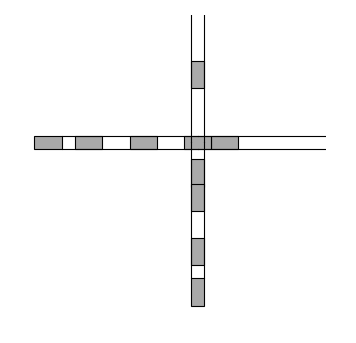
\includegraphics[width=0.4\textwidth]{figures/single/single_intersection_example.png}
  \caption{Illustration of a single intersection with vehicles drawn as grey
    rectangles. Vehicles approach the intersection from the east and from the
    south and cross it without turning. Note that the first two waiting vehicles
    on the south lane kept some distance before the intersection, such that they
    are able to reach full speed whenever they
    cross.}\label{fig:intersection_illustration}
\end{figure}

% model notation
Consider the single intersection illustrated in
Figure~\ref{fig:intersection_illustration}. Assume there are two incoming lanes,
identified by indices $\mathcal{R} = \{ 1, 2 \}$. The corresponding two routes
are crossing the intersection from south to north and crossing from west to
east. We identify vehicles by their route and by their relative order on this
route, by defining the vehicle index set
\begin{align}
  \mathcal{N} = \{ (r, k) : k \in \{1, \dots, n_{r}\}, r \in \mathcal{R}\} ,
\end{align}
where $n_{r}$ denotes the number of vehicles following route $r$. Smaller
values of $k$ correspond to reaching the intersection earlier. Given vehicle
index $i = (r, k) \in \mathcal{N}$, we also use the notation $r(i) = r$ and
$k(i) = k$.
%
We assume that each vehicle is represented as a rectangle of length $L$ and
width $W$ and that its position $x_{i}(t)$ is measured as the distance between
its front bumper and the start of the lane. In order to maintain a safe distance
between consecutive vehicle on the same lane, vehicle trajectories need to
satisfy
\begin{align}
  \label{eq:follow_constraints}
  x_{i}(t) - x_{j}(t) \geq L ,
\end{align}
for all $t$ and all pairs of indices $i, j \in \mathcal{N}$ such that
$r(i) = r(j), k(i) + 1 = k(j)$. Let $\mathcal{C}$ denote the set of such ordered
pairs of indices. Note that these constraints restrict vehicle from overtaking
each other, so the initial relative order is always maintained.
%
For each $i \in \mathcal{N}$, let $\mathcal{E}_{i} = (B_{i}, E_{i})$ denote the
open interval such that vehicle $i$ occupies the intersection's conflict area if
and only if $B_{i} < x_{i}(t) < E_{i}$. Using this notation, collision avoidance
at the intersection is achieved by requiring
\begin{align}
  \label{eq:conflict_constraints}
  (x_{i}(t), x_{j}(t)) \notin \mathcal{E}_{i} \times \mathcal{E}_{j} ,
\end{align}
for all $t$ and for all pairs of indices $i, j \in \mathcal{N}$ with
$r(i) \neq r(j)$, which we collect in the set $\mathcal{D}$.
%
Suppose we have some performance criterion $J(x_{i})$ that takes into account
travel time and energy efficiency of the trajectory of vehicle $i$, then the
offline trajectory optimization problem for a single intersection can be
compactly written as
\begin{subequations}
\label{eq:offline_single_intersection}
\begin{align}
  \min_{\mathbf{x}(t)} \quad & \sum_{i \in \mathcal{N}} J(x_{i}) \\
  \text{s.t.} \quad  & x_{i} \in D_{i}(s_{i,0}) , &\text{for all } i \in \mathcal{N} , \\
                & x_{i}(t) - x_{j}(t) \geq L, &\text{for all } (i,j) \in \mathcal{C} , \\
                & (x_{i}(t), x_{j}(t))  \notin \mathcal{E}_{i} \times \mathcal{E}_{j} , &\text{for all } \{i,j\} \in \mathcal{D} \label{eq:collision_constraints} ,
\end{align}
\end{subequations}
where $\mathbf{x}(t) = [\, x_{i}(t) : i \in \mathcal{N} \,]$ and constraints are
for all $t$.


\subsection{Direct transcription}

Although computationally demanding,
problem~\eqref{eq:offline_single_intersection} can be numerically solved by
direct transcription to a non-convex mixed-integer linear program by
discretization on a uniform time grid. Let $K$ denote the number of discrete
time steps and let $\Delta t$ denote the time step size.
%
Using the forward Euler integration scheme, we have
\begin{align*}
  x_{i}(t + \Delta t) = x_{i}(t) + v_{i}(t) \Delta t , \\
  v_{i}(t + \Delta t) = v_{i}(t) + u_{i}(t) \Delta t ,
\end{align*}
for each $t \in \{0, \Delta t, \dots, K \Delta t\}$. Following the approach
in~\cite{hultApproximateSolutionOptimal2015}, the collision-avoidance
constraints between lanes can be formulated using the well-known big-M technique
by the constraints
\begin{align*}
  x_{i}(t) \leq B_{i} + \delta_{i}(t) M , \\
  E_{i} - \gamma_{i}(t) M \leq x_{i}(t) , \\
  \delta_{i}(t) + \delta_{j}(t) + \gamma_{i}(t) + \gamma_{j}(t) \leq 3 ,
\end{align*}
where $\delta_{i}(t), \gamma_{i}(t) \in \{ 0, 1 \}$ for all $i \in \mathcal{N}$ and $M$ is a
sufficiently large number.
%
Finally, the follow constraints can simply be added as
\begin{align*}
  x_{i}(t) - x_{j}(t) \geq L ,
\end{align*}
for each $t \in \{0, \Delta t, \dots, K \Delta t\}$ and each pair of consecutive
vehicles $(i, j) \in \mathcal{C}$ on the same lane.
%
For example, consider the objective functional
\begin{align*}
  J(x_{i}) = \int_{t=0}^{t_{f}} \left( {(v_{d} - v_{i}(t))}^{2} + {u_{i}(t)}^{2} \right) dt ,
\end{align*}
where $v_{d}$ is some reference velocity and $t_{f}$ denotes the final time,
then the optimal trajectories are shown in
Figure~\ref{fig:direct_transcription_example}.

\definecolor{armygreen}{rgb}{0.29, 0.33, 0.13}
\begin{table}[H]
  \centering
\begin{tabular}{ c | c c c | c c }
  $i$  & {\color{armygreen}(1,1)} & {\color{armygreen}(1,2)} & {\color{armygreen}(1,3)} & {\color{red}(2,1)} & {\color{red}(2,2)} \\
  \hline
  $x_{i}(0)$ & 15 & 10 &  0 & 10 &  0 \\
  $v_{i}(0)$ & 10 & 10 &  6 & 12 & 10 \\
\end{tabular}
\caption{Example initial conditions $s_{i,0} = (x_{i}(0), v_{i}(0))$ for
  problem~\eqref{eq:offline_single_intersection}.}
\label{tab:hult_parameters}
\end{table}

\begin{figure}
  \centering
  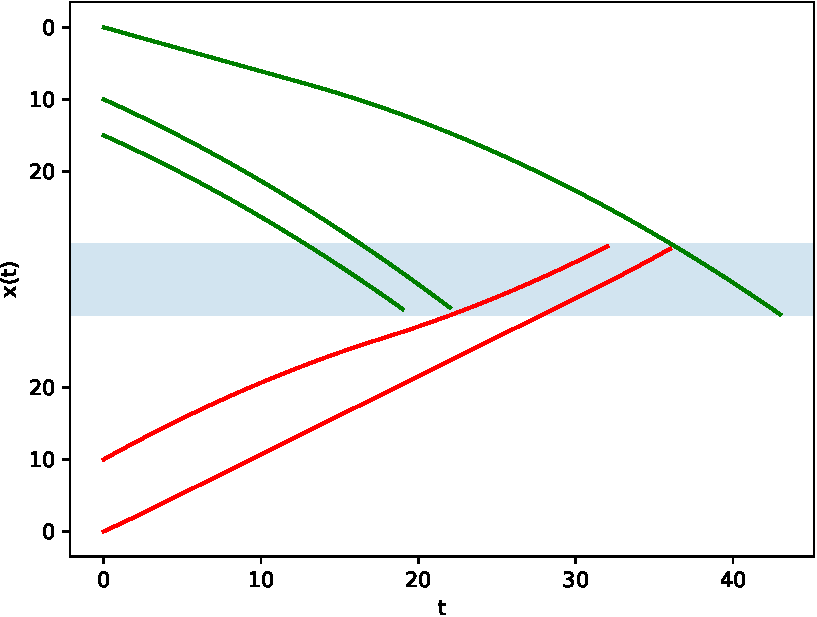
\includegraphics[width=0.8\textwidth]{figures/single/trajectories_general.pdf}
  \caption{Example of optimal trajectories obtained using the direct
    transcription method with
    $L = 5, \, \mathcal{E}_{i} \equiv \mathcal{E} = [50, 70], \, v_{d} = 20, \; T=120, \, \Delta t = 0.1$
    and initial conditions as given in Table~\ref{tab:hult_parameters}. The
    y-axis is split such that each part corresponds to one of the two lanes and
    the trajectories are inverted accordingly and drawn with separate colors.
    The intersection area $\mathcal{E}$ is drawn as a shaded region. Whenever a
    vehicle has left the intersection, we stop drawing its trajectory for
    clarity.}
  \label{fig:direct_transcription_example}
\end{figure}


\subsection{General decomposition}

For the case where only a single vehicle is approaching the intersection for
each route, so $n_{r} = 1$ for each route $r \in \mathcal{R}$, it has been shown
that problem~\eqref{eq:offline_single_intersection} can be decomposed into two coupled optimization problems, see
Theorem 1 in~\cite{hultApproximateSolutionOptimal2015}. Roughly speaking, the \textit{upper-level problem} optimizes the time
slots during which vehicles occupy the intersection, while the \textit{lower-level problem}
produces optimal safe trajectories that respect these time slots.
%
When allowing multiple vehicles per lane, we show without proof that a similar
decomposition is possible.
%
Given $x_{i}(t)$, the \textit{crossing time} of vehicle $i$, when the vehicle
first enters the intersection, and the corresponding \textit{exit time} are respectively
\begin{align*}
  \inf \{ t: x_{i}(t) \in \mathcal{E}_{i} \}  \;\; \text{ and } \; \sup \{ t: x_{i}(t) \in \mathcal{E}_{i} \} .
\end{align*}
%
The upper-level problem is to find a set of feasible occupancy timeslots, for
which the lower-level problem generates trajectories. We will use decision
variable $y(i)$ for the crossing time and write $y(i) + \sigma(i)$ for the exit
time. It turns out that trajectories can be generated separately for each route,
which yields the decomposition
%
\begin{align*}
  \min_{y, \sigma} \quad & \sum_{r \in \mathcal{R}} F(y_{r}, \sigma_{r}) \\
  \text{ s.t. } \quad & y(i) + \sigma(i) \leq y(j) \text{ or } y(j) + \sigma(j) \leq y(i), & \text{ for all } \{i, j\} \in \mathcal{D} , \\
  & (y_{r}, \sigma_{r}) \in \mathcal{S}_{r} , & \text{ for all } r \in \mathcal{R} ,
\end{align*}
where $F(y_{r}, \sigma_{r})$ and $\mathcal{S}_{r}$ are the value function and
set of feasible parameters, respectively, of the lower-level \textit{route trajectory optimization}
problem
\begin{align*}
  F(y_{r}, \sigma_{r}) = \min_{x_{r}} \quad & \sum_{i \in \mathcal{N}_{r}} J(x_{i}) \\
  \text{ s.t. } \quad & x_{i} \in D_{i}(s_{i,0}) , & \text{ for all } i \in \mathcal{N}_{r} , \\
  & x_{i}(y(i)) = B_{i} , & \text{ for all } i \in \mathcal{N}_{r} , \\
  & x_{i}(y(i) + \sigma(i)) = E_{i} , & \text{ for all } i \in \mathcal{N}_{r} , \\
  & x_{i}(t) - x_{j}(t) \geq L , & \text{ for all } (i, j) \in \mathcal{C} \cap \mathcal{N}_{r} ,
\end{align*}
where we used $\mathcal{N}_{r} = \{ i \in \mathcal{N} : r(i) = r \}$ and
similarly for $x_{r}, y_{r}$ and $\sigma_{r}$ to group variables according to
route. Note that the set of feasible parameters $\mathcal{S}_{r}$ implicitly
depends on the initial states $s_{r,0}$ and system parameters.


\subsection{Decomposition for delay objective}

Assume that the trajectory performance criterion is exactly the crossing time,
so $J(x_{i}) = \inf \{ t: x_{i}(t) \in \mathcal{E}_{i} \}$. This assumption
makes the problem significantly simpler, because we have
\begin{align*}
  F(y_{r}, \sigma_{r}) \equiv F(y_{r}) = \sum_{i \in \mathcal{N}_{r}} y(i) .
\end{align*}
%
Furthermore, we assume that vehicles enter the network and cross the
intersection at full speed, so $v_{i}(0) = v_{i}(y(i)) = v_{\max}$, such that we
have
\begin{align*}
\sigma(i) \equiv \sigma = (L + W) / v_{\max}, \; \text{ for all } i \in \mathcal{N} .
\end{align*}
%
Therefore, we ignore the part related to $\sigma$ in the set of feasible
parameters $\mathcal{S}_{r}$, which can be shown that to have a particularly
simple structure under these assumptions.
% earliest time of arrival
Observe that $a_{i} := (B_{i} - x_{i}(0)) / v_{\max}$ is the earliest time at
which vehicle $i$ can enter the intersection.
% processing time
Let $\rho := L / v_{\max}$ be such that $y(i) + \rho$ is the time at which
the rear bumper of a crossing vehicle reaches the start line of the
intersection.
We will refer to $a_{i}$ and $\rho$ as the \textit{arrival time} and \textit{processing time}, respectively.
It can now be shown that $y_{r} \in \mathcal{S}_{r}$ holds whenever
\begin{align*}
  a_{i} \leq y(i) , & \text{ for all } i \in \mathcal{N}_{r} , \\
  y(i) + \rho \leq y(j) , & \text{ for all } (i,j) \in \mathcal{C} \cap \mathcal{N}_{r} .
\end{align*}
Therefore, under the stated assumptions, the offline trajectory optimization
problem~\eqref{eq:offline_single_intersection} reduces to the following \textit{crossing time scheduling} problem
\begin{subequations}
  \label{eq:crossing_time_scheduling}
\begin{align}
  \min_{y} \quad & \sum_{i \in \mathcal{N}} y(i) \\
  \text{ s.t. } \quad & a_{i} \leq y(i) , & \text{ for all } i \in \mathcal{N} , \\
                    & y(i) + \rho \leq y(j) , & \text{ for all } (i,j) \in \mathcal{C} \label{eq:conjunctive} , \\
                    & y(i) + \sigma \leq y(j) \text{ or } y(j) + \sigma \leq y(i) , & \text{ for all } \{i,j\} \in \mathcal{D} \label{eq:disjunctive} .
\end{align}
\end{subequations}
This problem can be solved using off-the-shelf mixed-integer linear program solvers,
after encoding the \textit{disjunctive constraints}~\eqref{eq:disjunctive} using
the big-M technique, which we will demonstrate in
Section~\ref{sec:branch-and-cut}. Given optimal crossing time schedule $y^{*}$, any set of trajectories
$[x_{i}(t) : i \in \mathcal{N}]$ that satisfies
\begin{align*}
  x_{i} \in D_{i}(s_{i,0}) , \quad & \text{ for all } i \in \mathcal{N} , \\
  x_{i}(y^{*}(i)) = B_{i} , \quad & \text{ for all } i \in \mathcal{N} , \\
  x_{i}(y^{*}(i) + \sigma) = E_{i} , \quad & \text{ for all } i \in \mathcal{N} , \\
  x_{i}(t) - x_{j}(t) \geq L , \quad & \text{ for all } (i,j) \in \mathcal{C} ,
\end{align*}
forms a valid solution. These trajectories can be computed with an efficient
direct transcription method. Note that each route may be considered separately.
Therefore, trajectories can be computed by solving the time-discretized version
of the optimal control problem
%
\begin{align*}
\texttt{MotionSynthesize}(\tau, B, s_{0}, x') := \\
  {\arg\min}_{x: [0, \tau] \rightarrow \mathbb{R}} & \int_{0}^{\tau} |x(t)| dt \\
  \text{ s.t. } & \ddot{x}(t) = u(t) , &  \text{ for all } t \in [0, \tau] , \\
  & |u(t)| \leq a_{\max} , &  \text{ for all } t \in [0, \tau] , \\
  & 0 \leq \dot{x}(t) \leq v_{\max} , &  \text{ for all } t \in [0, \tau] , \\
  & x'(t) - x(t) \geq L , &  \text{ for all } t \in [0, \tau] , \\
  & (x(0), \dot{x}(0)) = s_{0} , \\
  & (x(\tau), \dot{x}(\tau)) = (B, v_{\max}) ,
\end{align*}
where $\tau$ is the required crossing time, $B$ denotes the distance to
the intersection, $s_{0}$ is the initial state of the vehicle and $x'$ denotes
the trajectory of the vehicle preceding the current vehicle.

\begin{figure}
  \centering
  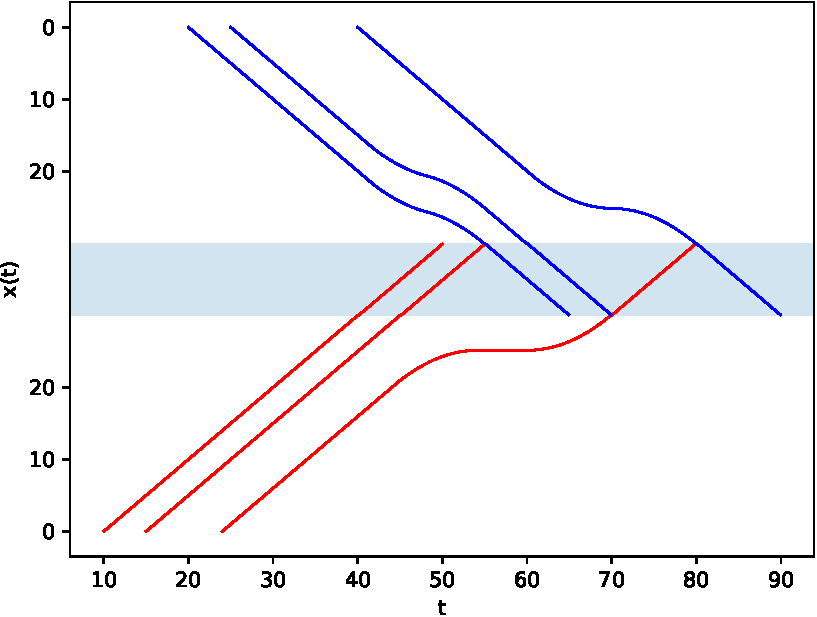
\includegraphics[width=0.8\textwidth]{figures/single/trajectories_delay.pdf}
  \caption{Example trajectories of vehicles from a single route, for some random
    arrival times and scheduled crossing times, computed by solving the linear
    program obtained from direct transcription of problem \texttt{MotionSynthesize}. We
    used the parameters $v_{\max} = 1, a_{\max} = 0.5, L = 5$. The ``queueing
    behavior'' that we also see in traffic jams is visible for the trajectories
    in the upper part. This is due to the particular choice of optimization
    objective, which essentially tries to keep all vehicles as close to the
    intersection as possible at all times.}
\end{figure}


\section{Crossing time scheduling}

Given a crossing time schedule $y$, trajectories can be efficiently computed
using a direct transcription method. Hence, we focus on solving the crossing
time scheduling problem~\eqref{eq:crossing_time_scheduling}. Before we start
discussing various solution techniques, let us first introduce an alternative
way of representing instances of~\eqref{eq:crossing_time_scheduling} by means of a
graph. Once we extend the current model to networks of intersection, this
encoding will be particularly helpful.

Instances and solutions of the crossing time optimization
problem~\eqref{eq:crossing_time_scheduling} can be represented by
their \textit{disjunctive graph}
$(\mathcal{N}, \mathcal{C}, \mathcal{O})$, which is a directed graph with nodes
$\mathcal{N}$ and the following two types of arcs. The \textit{conjunctive arcs}
encode the fixed order of vehicles driving on the same lane. For each
$(i,j) \in \mathcal{C}$, an arc from $i$ to $j$ means that vehicle $i$ reaches
the intersection before $j$ due to the follow
constraints~\eqref{eq:conjunctive}. The \textit{disjunctive arcs} are used to
encode the decisions regarding the ordering of vehicles from distinct lanes,
corresponding to constraints~\eqref{eq:disjunctive}. For each pair
$\{i,j\} \in \mathcal{D}$, at most one of the arcs $(i,j)$ and $(j,i)$ can be
present in $\mathcal{O}$.

When $\mathcal{O} = \varnothing$, we say the disjunctive graph is
\textit{empty}. Each feasible schedule satisfies exactly one of the two
constraints in~\eqref{eq:disjunctive}. When $\mathcal{O}$ contains exactly one arc from every pair
of opposite disjunctive arcs, we say the disjunctive graph is \textit{complete}.
Note that such graph is acyclic and induces a unique topological ordering $\pi$
of its nodes. Conversely, every ordering $\pi$ of nodes $\mathcal{N}$ corresponds
to a unique complete disjunctive graph, which we denote by
$G(\pi) = (\mathcal{N}, \mathcal{C}, \mathcal{O}(\pi))$.

% edge weights
We define weights for every possible arc in a disjunctive graph. Every
conjunctive arc $(i, j) \in \mathcal{C}$ gets weight $w(i,j) = \rho_{i}$ and every
disjunctive arc $(i, j) \in \mathcal{O}$ gets weight $w(i,j) = \sigma_{i}$. Given
some vehicle ordering $\pi$, for every $j \in \mathcal{N}$, we recursively define
the lower bound
\begin{align}
  \label{eq:lower_bounds}
  \beta(j) = \max\{ a_{j}, \max_{i \in N^{-}_{\pi}(j)} \beta(i) + w(i,j) \} ,
\end{align}
where $N^{-}_{\pi}(j)$ denotes the set of in-neighbors of node $j$ in $G(\pi)$.
Observe that this quantity is a lower bound on the crossing time, i.e., every
feasible schedule $y$ with ordering $\pi$ must satisfy $y_{i} \geq \beta(i)$
for all $i \in \mathcal{N}$.
%
As the following result shows, it turns out that this lower bound is actually tight for optimal schedules,
which allows us to calculate the optimal crossing times $y^{*}$ once we know an
optimal ordering $\pi^{*}$ of vehicles, so we can concentrate on finding the latter.

\begin{proposition}\label{prop:active-schedule}
  If $y$ is an optimal schedule
  for~\eqref{eq:crossing_time_scheduling} with ordering $\pi$, then
  \begin{align}
    \label{eq:optimality}
    y_{i} = \beta(i) \quad \text{ for all } i \in \mathcal{N} .
  \end{align}
\end{proposition}


\subsection{Branch-and-cut}
\label{sec:branch-and-cut}

Optimization problem~\eqref{eq:crossing_time_scheduling} can be turned into
a Mixed-Integer Linear Program (MILP) by rewriting the disjunctive constraints using
the well-known big-M method.
%
We introduce a binary decision variable $\gamma_{ij}$ for every
disjunctive pair $\{i, j\} \in \mathcal{D}$.
%
To avoid redundant variables, we first impose some arbitrary ordering of the
disjunctive pairs by defining
\begin{align*}
  \bar{\mathcal{D}} = \{ (i,j) : \{i,j\} \in \mathcal{D}, \; l(i) < l(j) \} ,
\end{align*}
such that for every $(i,j) \in \bar{\mathcal{D}}$, setting $\gamma_{ij} = 0$
corresponds to choosing disjunctive arc $i \rightarrow j$ and
$\gamma_{ij} = 1$ corresponds to $j \rightarrow i$. This yields the following
MILP formulation
%
\begin{align*}
  \min_{y} \quad & \sum_{i \in \mathcal{N}} y_{i} & \\
  \text{s.t.} \quad & a_{i} \leq y_{i} , & \text{ for all } i \in \mathcal{N} , \\
  & y_{i} + \rho \leq y_{j} , & \text{ for all } (i,j) \in \mathcal{C} , \\
  & y_{i} + \sigma \leq y_{j} + \gamma_{ij}M , & \text{ for all } (i,j) \in \bar{\mathcal{D}} , \\
  & y_{j} + \sigma \leq y_{i} + (1 - \gamma_{ij})M , & \text{ for all } (i,j) \in \bar{\mathcal{D}} , \\
  & \gamma_{ij} \in \{0, 1\} , & \text{ for all } (i,j) \in \bar{\mathcal{D}} ,
\end{align*}
where $M > 0$ is some sufficiently large number. Next, we will discuss two
types of cutting planes that can be added to this formulation, which we hope
improve the solving time.

Consider some disjunctive arc $(i,j) \in \bar{\mathcal{D}}$. Let
$\mathit{pred}(i)$ denote the set of indices of vehicles that arrive no later
than $i$ on route $r(i)$. Alternatively, we could say
these are all the vehicles from which there is a path of conjunctive arcs to
$i$. Similarly, let $\mathit{succ}(j)$ denote the set of indices of vehicles
that arrive no later than $j$ on route $r(j)$.
%
Now suppose $\gamma_{ij} = 0$, so the direction of the arc is $i \rightarrow j$,
then any feasible solution must also satisfy
\begin{align*}
  p \rightarrow q \equiv \gamma_{pq} = 0 \; \text{ for all } \; p \in \mathit{pred}(i), \; q \in \mathit{succ}(j) .
\end{align*}
Written in terms of the disjunctive variables, this gives us the following cutting planes
\begin{align*}
  \sum_{\substack{p \in \mathit{pred}(i)\\ q \in \mathit{succ}(j)}} \gamma_{pq} \leq \gamma_{ij} M ,
\end{align*}
for every disjunction $(i,j) \in \bar{\mathcal{D}}$. We refer to these as
the \textit{transitive cutting planes}.

% Under the condition that $\rho_{i} = \rho$ and $\sigma_{i} = \sigma > \rho$ for all $i \in \mathcal{N}$,

Apart from the redundancy that stems from the way the disjunctions are encoded,
the next proposition shows that there is some less obvious structure in the
problem. Roughly speaking, whenever a vehicle can be scheduled immediately after
its predecessor, this should happen in any optimal schedule. We will use these
necessary conditions to define two types of additional cutting planes.

\begin{restatable}{proposition}{Exhaustive}\label{prop:exhaustive}
  If $y$ is an optimal schedule for~\eqref{eq:crossing_time_scheduling},
  satisfying $y_{i^{*}} + \rho \geq a_{j^{*}}$ for some $(i^{*},j^{*}) \in \mathcal{C}$, then $j^{*}$
  follows immediately after $i^{*}$, so $y_{i^{*}} + \rho = y_{j^{*}}$.
\end{restatable}

In order to model this type of necessary condition, we introduce for every
conjunctive pair $(i,j) \in \mathcal{C}$ a binary variable $\delta_{ij} \in \{0, 1\}$ that
satisfies
\begin{align*}
  \delta_{ij} = 0 &\iff y_{i} + \rho < a_{j} , \\
  \delta_{ij} = 1 &\iff y_{i} + \rho \geq a_{j} ,
\end{align*}
which can be enforced by adding to the constraints
\begin{align*}
  y_{i} + \rho &< a_{j} + \delta_{ij}M , \\
  y_{i} + \rho &\geq a_{j} - (1 - \delta_{ij}) M .
\end{align*}
Now observe that Proposition~\ref{prop:exhaustive} for $(i,j)$ is modeled by the
cutting plane
\begin{align*}
  y_{i} + \rho &\geq y_{j} - (1 - \delta_{ij}) M .
\end{align*}
We refer to these cutting planes as \textit{necessary conjunctive cutting planes}.
%
Using the definition of $\delta_{ij}$, we can add more cutting planes on the
disjunctive decision variables, because whenever $\delta_{ij} = 1$, the directions of
the disjunctive arcs $i \rightarrow k$ and $j \rightarrow k$ must be the same for every other vertex
$k \in \mathcal{N}$. Therefore, consider the following constraints
\begin{align*}
  \delta_{ij} + (1 - \gamma_{ik}) + \gamma_{jk} \leq 2 , \\
  \delta_{ij} + \gamma_{ik} + (1 - \gamma_{jk}) \leq 2 ,
\end{align*}
for every $(i,j) \in \mathcal{C}$ and for every $k \in \mathcal{N}$ with $r(k) \neq r(i) = r(j)$.
We will refer to these types of cuts as the \textit{necessary disjunctive cutting planes}.

\subsection{Runtime analysis}

For each route $r \in \mathcal{R}$, we model the sequence of earliest crossing times
$a_{r} = (a_{r1}, a_{r2}, \dots)$ as a stochastic process, to which we refer as
the \textit{arrival process}. Recall that constraints~\eqref{eq:conjunctive}
ensure a safe following distance between consecutive vehicles on the same route.
Therefore, we want the process to satisfy
\begin{align*}
  a_{(r, k)} + \rho_{(r,k)} \leq a_{(r, k + 1)} ,
\end{align*}
for all $k = 1, 2, \dots$. We start by assuming that all vehicles share the same
dimensions so that $\rho_{i} = \rho$ for all $i \in \mathcal{N}$.
%
Let the interarrival times be denoted as $X_{n}$ with cumulative distribution
function $F$ and mean $\mu$, assuming it exists. We define the arrival times
$A_{n} = A_{n-1} + X_{n} + \rho$, for $n \geq 1$ with $A_{0} = 0$.
%
The arrival process may be interpreted as an renewal process with interarrivals
times $X_{n} + \rho$.
%
% To be precise, let $I_{t} \in \{0, 1\}$
% denote the state of the process at time $t$ and assume the process starts in
% state $I_{0} = 0$. Let $X_{1}, X_{2}, \dots$ denote the times spend in state $0$
% and let $\rho$ be the time spend in state $1$.
%
Let $N_{t}$ denote the corresponding counting process, then by the \textit{renewal
  theorem}, we obtain the \textit{limiting density} of arrivals
%
\begin{align*}
  \mathbb{E}(N_{t + h}) - \mathbb{E}(N_{t}) \rightarrow \frac{h}{\mu + \rho} \quad \text{ as } t \rightarrow \infty ,
\end{align*}
for $h > 0$. Hence, we refer to the quantity $\lambda := {(\mu + \rho)}^{-1}$ as the
arrival intensity.

%
% Given
% some time $t>0$, define the \textit{truncation} $a_{i}(t)$ as the finite
% subsequence $(a_{i1}, \dots, a_{ik})$ of $a_{i}$ such that $a_{ik} \leq t$.
% %
% Let $f^{*}(a_{1}(t), a_{2}(t))$ denote an optimal schedule for the crossing
% time scheduling problem with arrivals $a_{1}(t)$ and $a_{2}(t)$.
% %
% Given some schedule $y$, we say that it has a \textit{schedule renewal at
%   time} $t$ whenever there are two consecutive vehicles
% $(i, j) \in \mathcal{C}$ such that $t = y(i) + \sigma < y(j)$. Let $R(y)$ denote
% the total number of such renewals in schedule $y$. Now consider the following
% limit
% \begin{align*}
%   L = \lim_{t \rightarrow \infty} R(f^{*}(a_{1}(t), a_{2}(t))) .
% \end{align*}
% Whenever $L < \infty$, we say that the system is \textit{unstable}.
% Whenever $L = \infty$, we say the system is \textit{stable}.
%
% Because there is in general no simple expression for $f^{*}$, it is not possible
% to state a necessary and sufficient condition for stability like often done for
% queueing systems. {\color{Navy}Argue that renewals do not change under $f^{*}$.}

In order to model the natural occurence of platoons, we model $F$ as a mixture
of two random variables, one with a small expected value $\mu_{s}$ to model the gap
between vehicles within the same platoon and one with a larger expected value $\mu_{l}$ to
model the gap between vehicles of different platoons. For example, consider a
mixture of two exponentials, such that
\begin{align*}
  F(x) &= p ( 1 - e^{-x / \mu_{s}} ) + (1 - p) (1 - e^{-x / \mu_{l}}) , \\[0.2em]
  \mu &= p \mu_{s} + (1-p) \mu_{l} ,
\end{align*}
%
assuming $\mu_{s} < \mu_{l}$. Observe that the parameter $p$ determines
the average length of platoons.
%
Consider two intersecting routes, $\mathcal{R} = \{1, 2\}$, with arrival processes
$a_{1} = (a_{11}, a_{12}, \dots)$ and $a_{2} = (a_{21}, a_{22}, \dots)$, with
arrival intensities $\lambda^{(1)} = \lambda^{(2)}$.
%
We keep $\lambda_{s} = 0.5$ constant, and use
\begin{align*}
  \mu_{l}  = \frac{\mu - p \mu_{s}}{1 - p}
\end{align*}
to keep the arrival rate constant accross arrival distributions.

We now assess which type of cutting planes yields the overall best performance.
The running time of branch-and-cut is mainly determined by the total number of
vehicles in the instance. Therefore, we consider instances with two routes and
measure the running time of branch-and-cut as a function of the number of
vehicles per route.
%
In order to keep the total computation time limited, we set a time limit of 60
seconds for solving each instance. Therefore, we should be careful when
calculating the average running time, because some observations may correspond
to the algorithm reaching the time limit, in which case the observation is said
to be \textit{censored}. Although there are statistical methods to rigorously
deal censored data, we do not need this for our purpose of picking the best type
of cutting planes.
%
Figure~\ref{fig:running_time} shows the average (censored) running time for the
three types of cutting planes. Observe that the necessary conjunctive cutting
planes seem to lower the running time the most.


\begin{figure}
  \centering
  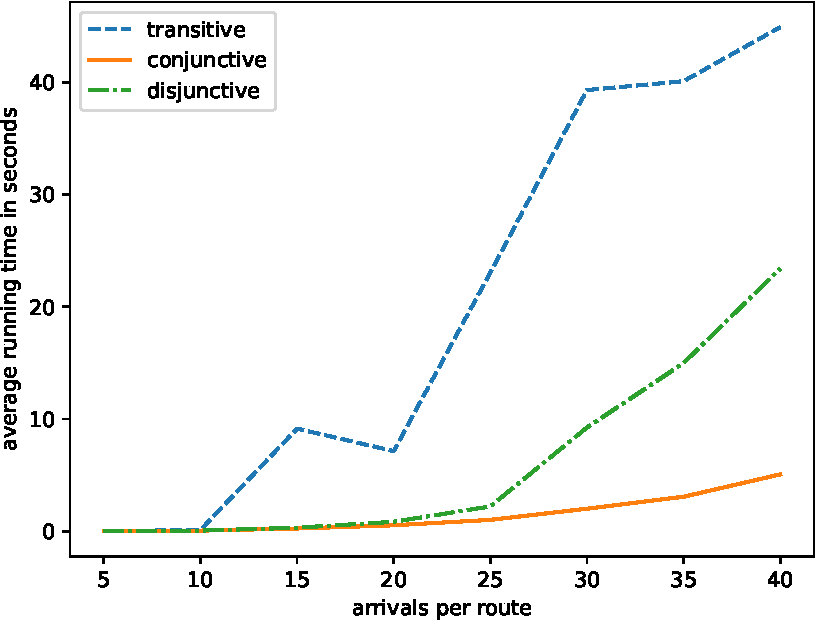
\includegraphics[width=0.7\textwidth]{data-single/running_times.pdf}
  \caption{The average (censored) running time of the branch-and-cut procedure
    is plotted as a function of the number of arriving vehicles per route, for
    each of the three indicated cutting planes. Each average is computed over
    $20$ problem instances. All instances use $\rho = 4$ and $\sigma = 1$. The arrivals
    of each of the two routes are generated using the bimodal exponential
    interarrival times with $p=0.5, \mu_{s} = 0.1, \mu_{l} = 10$. This figure
    clearly shows that the conjunctive cutting planes provide the most runtime
    improvement.}
  \label{fig:running_time}
\end{figure}


\section{Constructive heuristics}

% constructive scheduling
Methods that rely on the branch-and-cut framework are guaranteed to find an
optimal solution, but their running time scale very badly with increasing
instance sizes. Therefore, we are interested in developing heuristics to obtain
good approximations in reasonable time. A common approach for developing such
heuristics in the scheduling literature is to try and construct a good schedule
in a step-by-step fashion. For our crossing time scheduling problem, we will
consider methods to incrementally construct a vehicle ordering, to which we will
refer as \textit{constructive heuristics}.

% introduce partial ordering and automaton model
% In order to support to upcoming discussion, we first introduce some auxiliary
% concepts and notation.
%
In what follows, we will work with a partial ordering $\pi$, considered to be a
permutation of the set of scheduled vehicles, denoted as
$\mathcal{N}(\pi) \subset \mathcal{N}$.
%
% For each partial ordering $\pi$, the corresponding disjunctive graph $G(\pi)$ is
% incomplete, meaning that some of the disjunctive arcs have not yet been added.
% lane ordering automaton
Observe that ordering vehicles is equivalent to ordering the routes, due to the
conjunctive constraints, so we will define constructive heuristics in terms of
repeatedly choosing the next route. Hence, it may be helpful to model this
process as a deterministic finite-state automaton, where the set of route
indices acts as the input alphabet $\mathcal{R} = \{ 1, \dots, n \}$. Let $S$ denote
the state space and let $\delta: S \times \mathcal{R} \rightarrow S$ denote the transition function.
% states
Let $s$ denote an instance of crossing time scheduling problem~\eqref{eq:crossing_time_scheduling}. Formally, we
must consider $s$ to be a fixed part of the state, so it does not change with
transitions. The other part of the state is the current partial ordering $\pi$.
% transitions
Let $(s, \pi) \in S$ denote the current state and let $r \in \mathcal{R}$ denote the
next input. Let $i \in \mathcal{N} \setminus \mathcal{N}(\pi)$ denote the next unscheduled
vehicle on route $r$, then the system transitions to $(s, \pi \mdoubleplus i)$,
where we use $\mdoubleplus$ to denote sequence concatenation. If no such vehicle
exists, the transition is undefined.
%
We will use $\eta$ to denote a valid sequence of route indices, we let $y_{\eta}(s)$
denote the schedule that is obtained by executing $\eta$ on the automaton. We say
that route order $\eta$ is optimal whenever $y_{\eta}(s)$ is optimal. In the
following, we will use $\mathrm{obj}(y)$ to denote the objective value of
schedule $y$, which is just the sum of the crossing times of all the vehicles.

%
% multi-step transition
% With a little abuse of notation, let $\delta(s, \eta) = \delta(s_{0}, \eta)$ denote the
% state that we obtain after applying sequence $\eta$ to the automaton with initial
% state $s_{0} = (s, \varnothing)$, which generalizes the single step transition function by
% recursively defining
% \begin{align*}
%   \delta(s_{0}, \eta_{1:t}) = \delta(\delta(s_{0}, \eta_{1:t-1}), \eta_{t}) .
% \end{align*}
%
% Therefore, an input sequence $\eta$ of routes is called a \textit{valid route
%   order} whenever it is of length
% \begin{align*}
%   N = \sum_{r \in \mathcal{R}} n_{r}
% \end{align*}
% and contains precisely $n_r = |\{ i \in \mathcal{N} : r(i) = r \}|$ occurrences
% of route $r \in \mathcal{R}$.

Instead of trying to map an instance $s$ directly to some optimal route order, we consider
a mapping $p : S \rightarrow \mathcal{R}$ such that setting $s_{0} = (s, \varnothing)$ and repeatedly
evaluating
\begin{align*}
  s_{t} = \delta(s_{t-1}, p(s_{t-1}))
\end{align*}
yields a final state $s_{N}(s, \pi^{*})$, where $\pi^{*}$ is an optimal ordering and
$N = \sum_{r \in \mathcal{R}} n_{r}$ denotes the total number of steps required
to arrive at a final state.
%
Observe that such a mapping must exist, because we can always set
$p(s_{t}) = \eta^{*}_{t+1}$ for every step $t$, given some optimal lane order
$\eta^{*}$. However, we do not hope to find an explicit representation of $p$,
because it would in general be very complex, so our aim is to find good
approximations.

The approximations that we will propose are based on the the earliest crossing
times of the unscheduled vehicles at each state $s_{t}$. Note that definition
in~\eqref{eq:lower_bounds} still makes sense for partial orderings; the only
difference is that the corrsponding disjunctive graph $G(\pi)$ is not complete.
We will use $\beta_{t}$ to refer to the earliest crossing times,
using $t$ to emphasize its dependency on the current state $s_{t} = (s, \pi)$.


\subsection{Threshold heuristic}

We know from Proposition~\ref{prop:exhaustive} that whenever it is possible to schedule a vehicle
immediately after its predecessor on the same route, then this must be done in
any optimal schedule.
%
Based on this idea, we might think that the same holds true whenever a vehicle
can be scheduled \textit{sufficiently} soon after its predecessor. Although this
is not true in general, we can define a simple constructive heuristic based on
this idea.
%
For every route $r \in \mathcal{R}$, let $k(r)$ denote the number of vehicles
that have already been scheduled. Hence, let $i = (\eta_{t}, k(\eta_{t}))$
denote the vehicle that was scheduled in the last step of the automaton. We
define the \textit{threshold policy}
\begin{align*}
  p_{\tau}(s_{t}) = \begin{cases}
                \eta_{t} \quad &\text{ if } \beta_{t}(i) + \rho + \tau \geq a_{j} \text{ and } (i,j) \in \mathcal{C} , \\
                \texttt{next}(\eta_{t}) & \text{ otherwise, }
              \end{cases}
\end{align*}
for some threshold $\tau \geq 0$, where the expression $\texttt{next}(\eta_{t})$ represents some route
other than $\eta_{t}$ with unscheduled vehicles left.
%
Let $y_{\tau}(s)$ denote the schedule that is obtained by executing the
heuristic with threshold $\tau$ on some instance $s$. We pick the value of $\tau$
that minimizes the average empirical objective over some set of training
instances $\mathcal{X}$, by defining
%
\begin{align*}
  \hat{\tau} = \arg\min_{\tau \geq 0} \sum_{s \in \mathcal{X}} \textrm{obj}(y_{\tau}(s)) .
\end{align*}

With the specific choice $\tau = 0$, the threshold rule is related to the \textit{exhaustive policy}
for polling systems. More precisely, executing this threshold rule on the
automaton may be interpreted as running a discrete event simulation of a polling
system with an exhaustive polling policy.

\begin{figure}
  \centering
  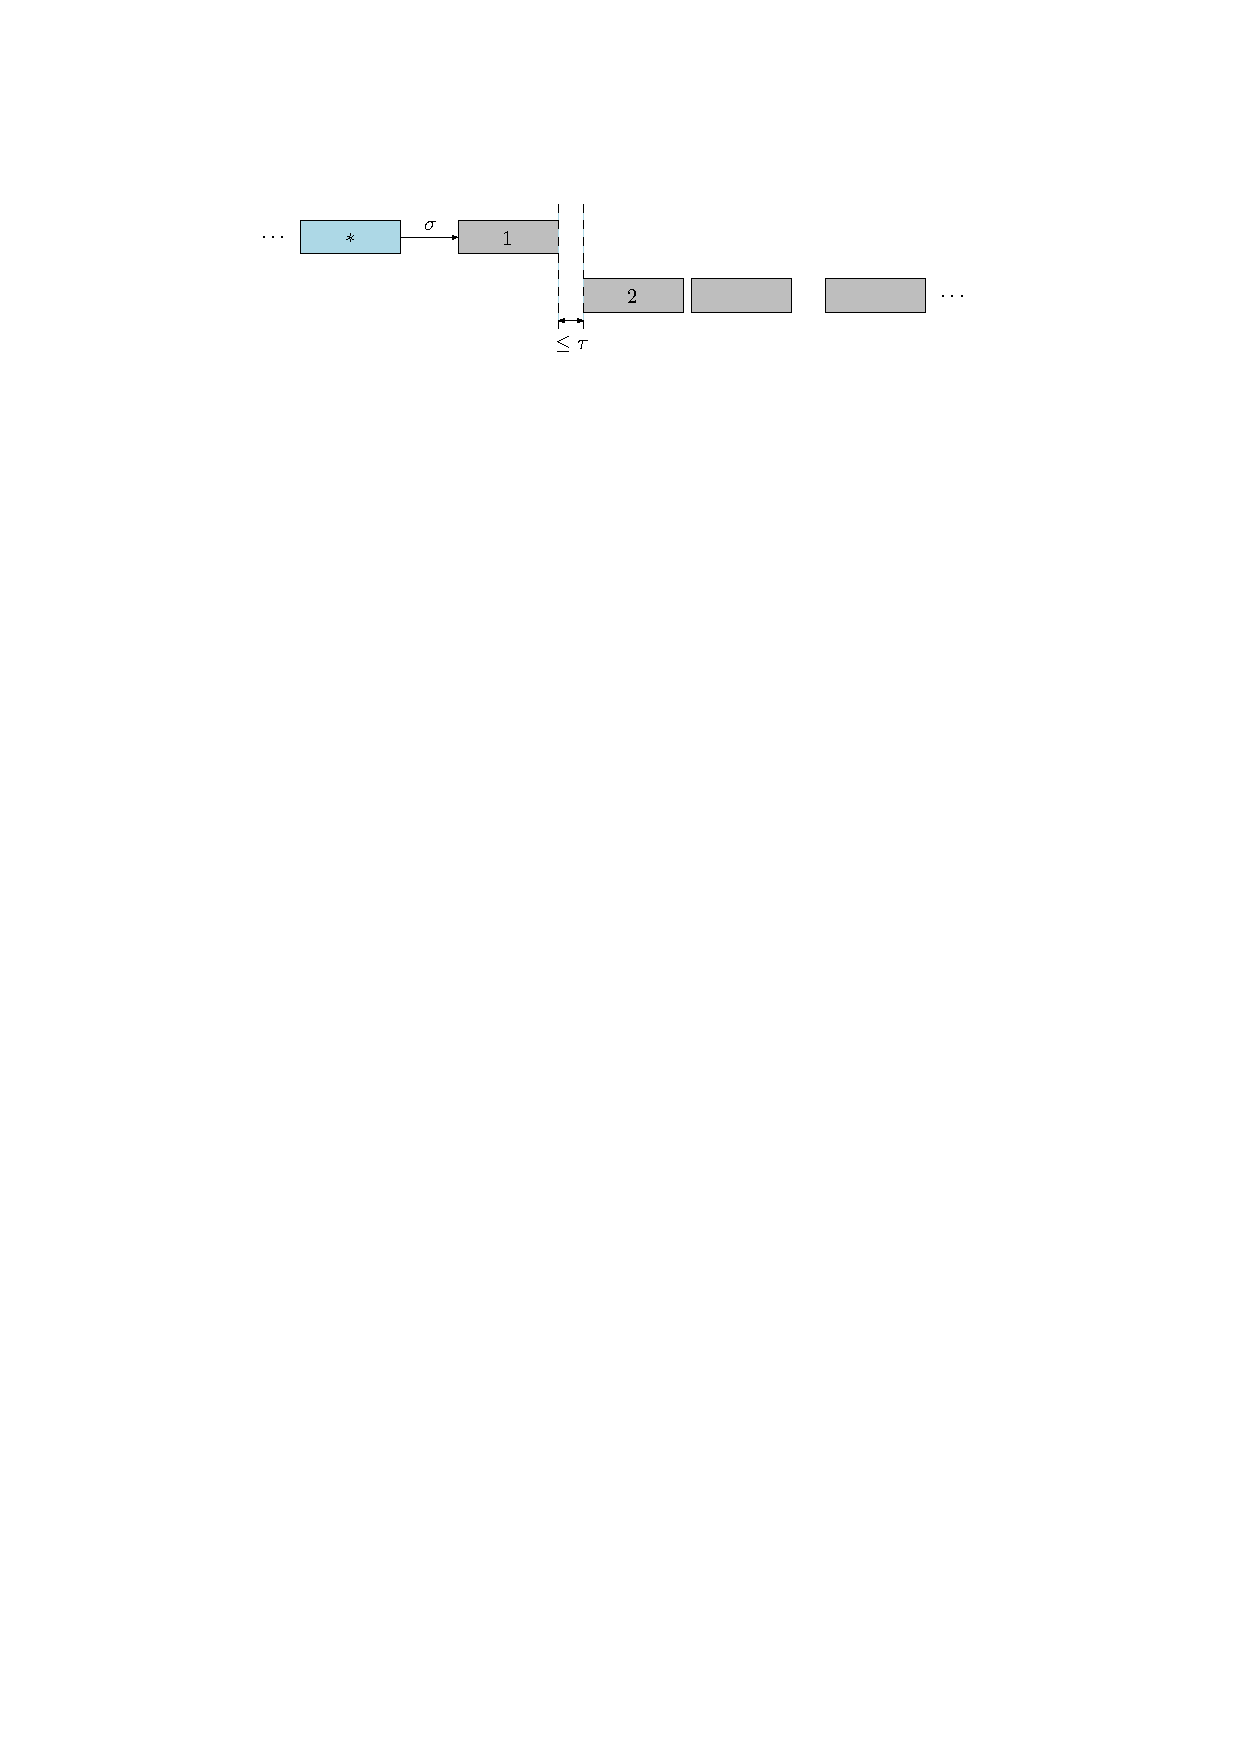
\includegraphics[width=0.9\textwidth]{figures/single/threshold}
  \caption{Illustration of the threshold heuristic for a specific situation
    during scheduling. The upper row represents the current partial schedule,
    where the vehicle marked with $*$ is from route 1, whereas all other
    vehicles are from route 2. Hence, the arrow indicates the switch time $\sigma$.
    The bottom row shows each unscheduled vehicles $i$ of route 2, placed at the
    earliest crossing times $\beta_{t}(i)$. Whenever the indicated distance is
    smaller than $\tau$, the threshold rule requires vehicle $2$ to be scheduled
    next.}\label{fig:threshold_heuristic}
\end{figure}


\subsection{Neural heuristic}
\label{sec:neural}

We will now consider a class of heuristics that directly generalizes the
threshold heuristic. Instead of looking at the earliest crossing time of the
next vehicle in the current lane, we will now consider the earliest arrival
times of all unscheduled vehicles across lanes.
%
Because we want to tune the heuristic based on problem instances, we will
formulate it as a model of the conditional probability
$p_{\theta}(\eta_{t+1} | s_{t})$ of the next route, given the current partial
order. Here, $\theta$ denotes the parameters that need to tuned to the specific class
of problem instances.


We will first explain how we parameterize $p_{\theta}$ as a function of the
current non-final state $s_{t} = (s, \pi_{t})$ of the automaton.
%
In the following definitions, the dependence on $s_{t}$ will be left implicit
to avoid cluttering the notation and we let $k(r)$ denote again the number of
scheduled vehicles of route $r$. Observe that the overall earliest arrival time
of any unscheduled vehicle in the system is given by
\begin{align*}
  T = \min_{r \in \mathcal{R}} \beta(r, k(r) + 1) .
\end{align*}
We define the \textit{horizon} of route $r$ to be the sequence of relative lower bounds
\begin{align*}
  h(r) = (\beta(r, k(r) + 1) - T, \beta(r, k(r) + 2) - T, \dots, \beta(r, n_{r}) - T) .
\end{align*}
%
Next, we compute for each horizon an embedding $\bar{h}(r)$.
%
Observe that horizons can be of arbitrary dimension. Therefore, we could
restrict each horizon to a fixed length by using zero padding.
%
To avoid the zero padding operation, which can be problematic for states that
are almost done, we employ a recurrent neural network for variable-length
sequences, to obtain a model that is agnostic to the number of remaining
unscheduled vehicles. Each horizon $h(r)$ is simply transformed into a
fixed-length embedding by feeding it in reverse order through a plain Elman RNN.
Generally speaking, the most recent inputs tend to have greater influence on the
output of an RNN, which is why we feed the horizon in reverse order, such that
those vehicles that are due first are processed last, since we expect those
should have the most influence on the decision.
%
Finally, the horizon embeddings are arranged into a vector $H$, defined as
\begin{align*}
  {H}_{r} = \bar{h}(r - \eta_{t} \; \mathrm{mod} \; |\mathcal{R}|) ,
\end{align*}
for every $r \in \mathcal{R}$, with $\eta_{t}$ denoting the current route (of the
last scheduled vehicle). By employing this kind of \textit{cycling trick}, we make sure
that the embedding of the current route is always kept at the same position of
the vector.
%
Using some fully connected neural network $f$, this global embedding is mapped to
the probability distribution $p_{\theta}(\eta_{t+1} | s_{t}) = f(H(s_{t}))$.

Note that the above model depends on the parameters of $f$ and possibly on the
parameters of the embedding, when using the recurrent approach. Let $\theta$
denote the vector of all these parameters.
% fitting
Consider an instance $s$ and some optimal route sequence $\eta$ with
corresponding states defined as $s_{t+1} = \delta(s_{t}, \eta_{t+1})$. The
resulting set of pairs $\mathcal{X} := \{ (s_{t}, \eta_{t+1}) : t = 1, \dots, N \}$ can be used to learn $p_{\theta}$
in a supervised fashion by treating it as a classification task and computing the maximum likelihood estimator $\hat{\theta}$.
%
We make this concrete for the case of two routes $\mathcal{R} = \{ 1, 2\}$.
Let $p_{\theta}(s_{t})$ denote the probability of choosing the first route and use the
binary cross entropy loss, defined as
\begin{align*}
  L_{\theta}(\mathcal{X}) = - \frac{1}{|\mathcal{X}|} \sum_{(s_{t}, \eta_{t+1}) \in \mathcal{X}} \mathds{1}\{\eta_{t+1} = 1\} \log(p_{\theta}(s_{t})) + \mathds{1}\{\eta_{t+1} = 2\} \log(1 - p_{\theta}(s_{t})) ,
\end{align*}
where $\mathds{1}\{\cdot\}$ denotes the indicator function. Now we can simply rely on
some (stochastic) gradient-descent optimization method to determine
\begin{align*}
  \hat{\theta} = \arg\min_{\theta} L_{\theta}(\mathcal{X}) .
\end{align*}

% inference
Once we determined the model parameters, schedules can be generated by employing
greedy inference as follows. The model $p_{\theta}$ provides a distribution over
lanes. We ignore lanes that have no unscheduled vehicles left and take the
argmax of the remaining probabilities. We will denote the corresponding complete
schedule by $\hat{y}_{\theta}(s)$.

\begin{figure}
  \centering
  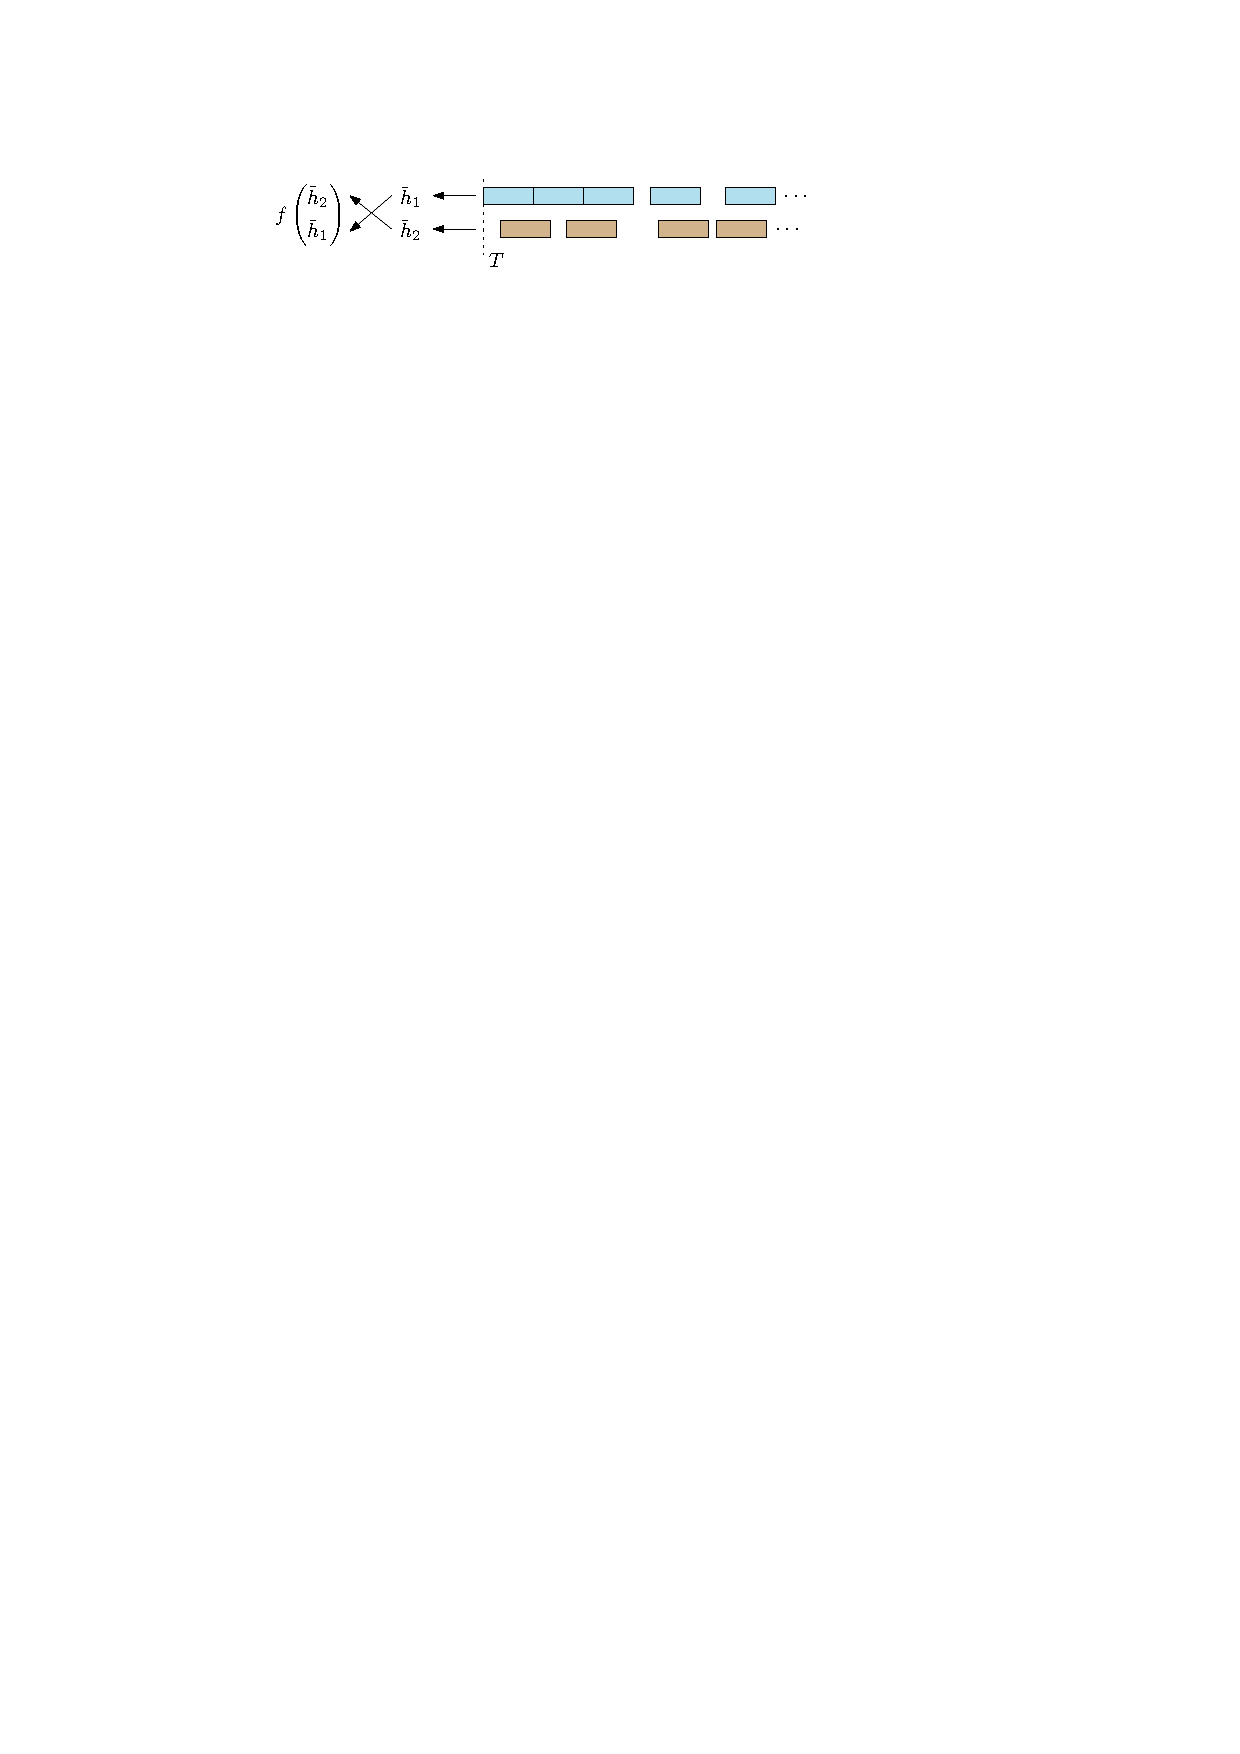
\includegraphics[width=0.9\textwidth]{figures/single/embedding}
  \caption{Schematic overview of how
    $p_{\theta}(\eta_{t+1} | s_{t}) = f(H(s_{t}))$, the conditional distribution
    over the next route to be chosen, is computed from the current route
    horizons via embedding and the cyling trick. Observe that this particular
    cycling corresponds to a situation in which the current route is
    $\eta_{t} = 2$.}\label{fig:neural_embedding}
\end{figure}


\subsection{Performance evaluation}

The assessment of the various solution methods is roughly based on two
aspects. Of course, the quality of the produced solutions is important. Second,
we need to take into account the time that the algorithm requires to compute the
solutions. We need to be careful about reporting the time requirements of the
constructive heuristics, because they need both training time as well as
inference time. Only reporting the latter time does not provide a fair
comparison.

We consider several problem instance distributions, because these may possibly
affect the performance of algorithms. The most important aspects that
characterize the distribution of problem instances are number of routes and
number of arrivals per route, distribution of interarrival times, arrival
intensity per route and degree of platooning.

We will refer to the total number of vehicles in an instance as its \textit{size}.
%
In the following, let $\mathcal{X}$ and $\mathcal{Y}$ denote a set of \textit{training instances}
and \textit{test instances}, respectively.
%
To enable a fair comparison across different instance classes, we report the
quality of a solution in terms of the average delay divided by the
instance size. More precisely, from now on we define the objective of some schedule $y$ as
\begin{align*}
  \textrm{obj}(y) = \frac{1}{|\mathcal{N}|} \sum_{i \in \mathcal{N}} y_{i} - a_{i} .
\end{align*}
%
Ideally, we want to report the average \textit{approximation ratio} of each
heuristic, which we define as
\begin{align*}
  \alpha_{\text{approx}} = \frac{1}{|\mathcal{Y}|} \sum_{s \in \mathcal{Y}} \frac{\textrm{obj}(\hat{y}(s)) - \textrm{obj}(y^{*}(s))}{\textrm{obj}(y^{*}(s))} ,
\end{align*}
where $y^{*}(s)$ denotes some optimal solution for instance $s$ and $\hat{y}(s)$
denotes some solution computed by a heuristic fitted to $\mathcal{X}$.
%
Again, we use a fixed time limit of 60 seconds per instance to bound the total
computation time of the analysis. Therefore, it might be that we cannot compute $y^{*}(s)$ using
the branch-and-cut procedure for some of the larger instances.
%
Instead of reporting the actual approximation ratio $\alpha_{\text{approx}}$, we
report the approximation ratio computed using the best solution that
branch-and-cut obtains within the time limit as proxy for $y^{*}(s)$.

The heuristics can be fitted to the training data without requiring much manual tweaking.
%
The threshold heuristics is fitted by choosing the best value of $\tau$ from a fixed set of candidates through a simple search.
The neural heuristics is trained for a fixed number of training steps. At regular intervals, we compute the average validation loss and store the current model parameters. At the end of the training, we pick the model parameters with the smallest validation loss.
%
We create some plots that allow us to manually inspect the model fit.
For the threshold heuristics, we plot the average objective for the values of
$\tau$ in the grid search, see Figure~\ref{fig:tau_fit}.
%
For the neural heuristic, we plot the training and validation loss, see
Figure~\ref{fig:neural_fit}. It can be seen that the model converges very steadily in all cases.

% silent package loading


\begin{knitrout}
\definecolor{shadecolor}{rgb}{0.969, 0.969, 0.969}\color{fgcolor}\begin{table}
\centering
\caption{\label{tab:results}Average scaled optimal objective value computed using MILP and using the threshold heuristic with threshold $\tau = 0$. Each class of problem instances is identified by the number $n$ of vehicle arrivals per route and the grid network size as cols x rows.}
\centering
\resizebox{\ifdim\width>\linewidth\linewidth\else\width\fi}{!}{
\begin{tabular}[t]{cc|cc|c|c|c|ccc|cc|c|c|c|ccc|cc|c|c|c|ccc|cc|c|c|c|ccc|cc|c|c|c|ccc|cc|c|c|c|ccc|cc|c|c|c|ccc|cc|c|c|c|c}
\toprule
n & size & MILP & time & $\tau = 0$  (gap) & random (gap) & boundary (gap) & alternate (gap)\\
\midrule
5 & 2x1 & 57.27 & 0.06 & 65.27 (11.45\%) & 58.96 (2.95\%) & 58.72 (2.52\%) & 58.23 (1.66\%)\\
5 & 3x1 & 57.67 & 0.12 & 68.34 (15.44\%) & 59.77 (3.65\%) & 59.82 (3.74\%) & 58.72 (1.83\%)\\
5 & 3x2 & 57.35 & 1.38 & 69.17 (18.32\%) & 60.88 (6.16\%) & 60.36 (5.25\%) & 58.82 (2.56\%)\\
\bottomrule
\end{tabular}}
\end{table}

\end{knitrout}


\section{Local search}

The previous section showed that constructive heuristics perform reasonably well
on average and sometimes even produce optimal solutions. To further increase
optimality of the heuristic solutions, without relying on systematic search
methods like branch-and-bound, we can try to use some kind of local search.
Specifically, compute a solution using one of the methods from the previous
section and then explore some \textit{neighboring solutions}, that we define next.

As seen in the previous sections, vehicles of the same route occur mostly in
groups, to which we will refer as \textit{platoons}. For example, consider for example
the route order $\eta = (0, 1, 1, 0, 0, 1, 1, 1, 0, 0)$. This example has 5
platoons of consecutive vehicles from the same route. The second platoon
consists of two vehicles from route 1.
%In general, let $P(\eta)$ denote the total number of platoons in $\eta$.
The basic idea is to make little changes in these platoons by moving vehicles at
the start and end of a platoon to the previous and next platoon of the same
route.
%
More precisely, we define the following two types of modifications to a route
order. A \textit{right-shift} modification of platoon $i$ moves the last vehicle of this
platoon to the next platoon of this route. Similarly, a \textit{left-shift} modification
of platoon $i$ moves the first vehicle of this platoon to the previous platoon
of this route.
%
We construct the neighborhood of a solution by performing every possible
right-shift and left-shift with respect to every platoon in the route order. For
illustration purposes, we have listed a full neighborhood for some example route
order in Table~\ref{tab:local_search}.

Now using this definition of a neighborhood, we must specify how the search
procedure visits these candidates.
In each of the following variants, the value of each neighbor is always computed.
%
The most straightforward way is to select the single best candidate in the
neighborhood and then continue with this as the current solution and compute its
neighborhood. This procedure can be repeated for some fixed number of times.
Alternatively, we can select the $k$ best neighboring candidates and then
compute the combined neighborhood for all of them. Then in the next step, we
again select the $k$ best candidates in this combined neighborhood and repeat.
The latter variant is sometimes referred to as \textit{beam search}.

\newcommand*{\1}{{\color{blue}1}}%
\newcommand*{\0}{{\color{red}0}}%

\begin{table}
\begin{center}
\begin{tabular}{c|c|c}
  platoon id  & left-shift & right-shift \\
  1 &  & (\1, \1, \0, \0, \0, \1, \1, \1, \0, \0) \\
  2 & (\1, \0, \1, \0, \0, \1, \1, \1, \0, \0) & (\0, \1, \0, \0, \1, \1, \1, \1, \0, \0) \\
  3 & (\0, \0, \1, \1, \0, \1, \1, \1, \0, \0) & (\0, \1, \1, \0, \1, \1, \1, \0, \0, \0) \\
  4 & (\0, \1, \1, \1, \0, \0, \1, \1, \0, \0) & (\0, \1, \1, \0, \0, \1, \1, \0, \0, \1) \\
  5 & (\0, \1, \1, \0, \0, \0, \1, \1, \1, \0) &
\end{tabular}
\end{center}
\caption{Neighborhood of route order $\eta = (\0, \1, \1, \0, \0, \1, \1, \1, \0, \0)$.}
\label{tab:local_search}
\end{table}


% \subsection{Regeneration theorem}

% It has been observed that some optimal schedules seem to \textit{decompose} into
% parts, whenever the crossing times of consecutive vehicles are sufficiently far
% apart~\cite{limpensOnlinePlatoonForming2023}.

% \begin{proposition}
%   Let $s$ be an instance of crossing time scheduling problem~\eqref{eq:crossing_time_scheduling}.
% \end{proposition}




\bibliography{references}
\bibliographystyle{ieeetr}


\newpage

\appendix

\section{Proof of Proposition~\ref{prop:exhaustive}}

First, we prove the following lemma that provides an easier expression for
calculating the lower bounds.

\begin{lemma}\label{lb_lemma}
  Let $\pi$ be some permutation of $\mathcal{N}$. Assume that
  $\sigma_{i} = \rho_{i} + s$, for every $i \in \mathcal{N}$, with $s > 0$.
  Consider a pair $i,j \in \mathcal{N}$ such that $i$ is the immediate predecessor
  of $j$ in $\pi$, so $\pi^{-1}(i) + 1 = \pi^{-1}(j)$, then
\begin{align}
  \label{eq:lb_lemma}
  \text{\upshape LB}_\pi(j) = \max \{ r_{j}, \text{\upshape LB}_\pi(i) + w(i, j) \} .
\end{align}
\end{lemma}
\begin{proof}
  Suppose $(i,j) \in \mathcal{C}$, see Figure~\ref{fig:lb_lemma},
  then the incoming disjunctive arcs of $j$ are
  $N^{-}_{\pi}(j) \setminus \{ i \} \subset N^{-}_{\pi}(i)$. Therefore, we have
  \begin{align*}
    \max_{v \in N^{-}_{\pi}(j) \setminus \{i\}} \text{LB}_\pi(v) + \sigma_{v} \leq \text{LB}_\pi(i) ,
  \end{align*}
  so that
      $\text{LB}_\pi(v) + w(v,j) \leq \text{LB}_\pi(i) + w(i,j)$
  for all $v \in N_{\pi}^{-}(j)$.

  Otherwise, we have $(i, j) \in \mathcal{O}(\pi)$.
  %
  Let $v \in \mathcal{N}$ such that $(v, j)$ is an arc.
  If $(v,j) \in \mathcal{C}$, then we have
  \begin{align*}
    \text{LB}_\pi(v) + w(v,j) =
    \text{LB}_\pi(v) + \rho_{v} \leq \text{LB}_\pi(v) + \sigma_{v} + \sigma_{i} \leq \text{LB}_\pi(i) + w(i,j) ,
  \end{align*}
  where the second inequality follows from $(v,i) \in \mathcal{O}(\pi)$.
  %
  If $(v, j) \in \mathcal{O}(\pi)$ with $l(v) \neq l(i)$, then $(v,i) \in \mathcal{O}(\pi)$, so
  \begin{align*}
    \text{LB}_\pi(v) + w(v, j) = \text{LB}_\pi(v) + w(v, i) \leq \text{LB}_\pi(i) \leq \text{LB}_\pi(i) + w(i,j) .
  \end{align*}
  If $(v, j) \in \mathcal{O}(\pi)$ with $l(v) = l(i)$, then there is a path of conjunctive arcs between $v$ and
  $i$, so we must have $\text{LB}_\pi(v) + \rho_{v} \leq \text{LB}_\pi(i)$.
  Furthermore, from $w(v,j) = \sigma_{v} = \rho_{v} + s$ follows that
  \begin{align*}
    \text{LB}_\pi(v) + w(v,j) = \text{LB}_\pi(v) + \rho_{v} + s \leq \text{LB}_\pi(i) + s \leq \text{LB}_\pi(i) + w(i, j) .
  \end{align*}

  To conclude, we have shown that
  $\text{LB}_\pi(v) + w(v,j) \leq \text{LB}_\pi(i) + w(i,j)$ for any
  $v \in N^{-}_{\pi}(j)$, from which statement~\eqref{eq:lb_lemma} follows.
\end{proof}

\begin{figure}
  \centering
  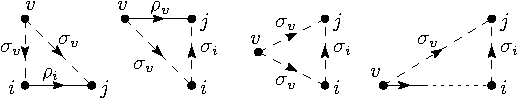
\includegraphics[width=0.9\textwidth]{figures/single/lower-bound-lemma.pdf}
  \caption{Sketch of the four cases distinguished in the proof of
    Lemma~\ref{lb_lemma}. Arc weights are given and disjunctive arcs
    $\mathcal{O}(\pi)$ are drawn with a dashed line.}\label{fig:lb_lemma}
\end{figure}


% \begin{proposition}
%   Consider an instance of~\eqref{eq:crossing_time_scheduling} with
%   $\rho_{i} = \rho$ and $\sigma_{i} = \sigma > \rho$ for all
%   $i \in \mathcal{N}$. Suppose $y$ is an optimal schedule with
%   $y_{i^{*}} + \rho \geq r_{j^{*}}$, for some $(i^{*},j^{*}) \in \mathcal{C}$,
%   then $j^{*}$ follows immediately after $i^{*}$, so
%   $y_{i^{*}} + \rho = y_{j^{*}}$.
% \end{proposition}

\Exhaustive*
\begin{proof}
  Suppose the ordering $\pi$ of $y$ is such that
  $\pi^{-1}(i^{*}) + 1 < \pi^{-1}(j^{*})$.
  %
  Let $\mathcal{I}(i,j) = \{ i, \pi(\pi^{-1}(i) + 1), \dots, j \}$ be the set of
  vehicles between $i$ and $j$.
  %
  Let $f = \pi(1)$ and $e = \pi(|\mathcal{N}|)$ be the first and last vehicles,
  respectively, and set $u = \pi^{-1}(i^{*}) + 1$ and $v = \pi^{-1}(j^{*}) - 1$, see also Figure~\ref{fig:platoon-preservation-diagram}.
  Construct new ordering $\pi'$ by moving vehicle $j^{*}$ forward
  by $|\mathcal{I}(u,v)|$ places and let $y'$ denote the corresponding schedule.
  %
  We have $y_{i} = y'_{i}$ for all $i \in \mathcal{I}(f, i^{*})$, so these do not
  contribute to any difference in the objective.
  %
  Using Proposition~\ref{prop:active-schedule} and Lemma~\ref{lb_lemma}, we compute
  \begin{align*}
    y'_{j^{*}} &= \max \{ r_{j^{*}}, y_{i^{*}} + \rho \} = y_{i^{*}} + \rho , \\
    y_{u} &= \max \{ r_{u}, y_{i^{*}} + \sigma \} , \\
    y'_{u} &= \max \{ r_{u}, y_{i^{*}} + \rho + \sigma \} ,
  \end{align*}
  where we used that $y_{i^{*}} + \rho \geq r_{j^{*}}$ by assumption.
  %
  Note that we have
  $y_{i^{*}} + \sigma + (|\mathcal{I}(u,v)| - 1) \rho \leq y_{v}$, regardless of the
  type of arcs between consecutive vehicles in $\mathcal{I}(u,v)$. Therefore,
  \begin{align*}
    y_{j^{*}} - y'_{j^{*}} \geq y_{v} + \sigma - y_{i^{*}} - \rho \geq 2 \sigma + (|\mathcal{I}(u,v)| - 2) \rho .
  \end{align*}

  We now show that $y'_{k} \geq y_{k}$ and $y'_{k} - y'_{j^{*}} \leq y_{k} - y_{i^{*}}$ for every $k \in \mathcal{I}(u,v)$.
  For $k = u$, it is clear that $y'_{u} \geq y_{u}$ and
  \begin{align*}
    y'_{u} - y'_{j^{*}} = \max \{ r_{u} - (y_{i^{*}} + \rho), \sigma \} \leq \max \{ r_{u} - y_{i^{*}}, \sigma \} = y_{u} - y_{i^{*}}.
  \end{align*}
  Now proceed by induction and let $x$ be the immediate predecessor of $k$ for
  which the inequalities hold, then
  \begin{align*}
    y'_{k} = \max \{ r_{k}, y'_{x} + w(x,k) \} \geq \max \{ r_{k}, y_{x} + w(x,k) \} = y_{k}
  \end{align*}
  and the second inequality follows from
  %\begin{align*}
  %  y'_{k} - y'_{x} = \max \{ r_{k} - y'_{x}, w(x,k) \} &\leq \max \{ r_{k} - y_{x}, w(x,k)\} = y_{k} - y_{x}
  %\end{align*}
  %implies that
  %\begin{align*}
  %  y'_{k} - y'_{j^{*}} = (y'_{k} - y'_{x}) + (y'_{x} - y'_{j^{*}}) \leq (y_{k} - y_{x}) + (y_{x} - y_{i^{*}}) = y_{k} - y_{i^{*}} .
  %\end{align*}
  %
  \begin{align*}
    (y'_{k} - y'_{x}) + (y'_{x} - y'_{j^{*}}) &= \max \{ r_{k} - y'_{x}, w(x,k) \} + (y'_{x} - y'_{j^{*}}) \\
                                             &\leq \max \{ r_{k} - y_{x}, w(x,k) \} + (y_{x} - y_{i^{*}}) \\
                                             &= (y_{k} - y_{x}) + (y_{x} - y_{i^{*}}) .
  \end{align*}

  Let $l$ denote the immediate successor of $j^{*}$, if there is one. Regardless of
  whether $j^{*}$ and $l$ are in the same lane, we have
  $y_{j^{*}} + \rho \leq y_{l}$. We derive
  \begin{align*}
    y'_{v} = y'_{v} - y'_{j^{*}} + y'_{j^{*}} \leq y_{v} - y_{i^{*}} + y'_{j^{*}} = y_{v} + \rho \leq y_{j^{*}} - \sigma + \rho ,
  \end{align*}
  from which follows that $y'_{v} + \sigma \leq y_{l}$,
  %\begin{align*}
  %  y'_{v} + \sigma = (y'_{v} - y'_{j^{*}}) + y'_{j^{*}} + \sigma \leq y_{v} - y_{i^{*}} + y'_{j^{*}} + \sigma = y_{v} + \rho + \sigma \leq y_{j^{*}} + \rho \leq y_{l} ,
  %\end{align*}
  which means that $y_{i} \geq y'_{i}$ for $i \in \mathcal{I}(l, e)$.

  We can now compare the objectives by putting everything together
  \begin{align*}
    \sum_{i \in \mathcal{N}} y_{i} - y'_{i} &=  y_{j^{*}} - y'_{j^{*}} + \sum_{i \in \mathcal{I}(u, v)} y_{i} - y'_{i} + \sum_{i \in \mathcal{I}(l, e)} y_{i} - y'_{i} \\
    &\geq 2 \sigma + (|\mathcal{I}(u,v)| - 2) \rho + \sum_{k \in \mathcal{I}(u,v)} (y_{k} - y_{i^{*}}) - (y'_{k} - y'_{j^{*}}) \\ & \hspace{12em} - |\mathcal{I}(u,v)| (y'_{j^{*}} - y_{i^{*}}) \\
    &\geq 2 \sigma - 2 \rho > 0
  \end{align*}
  which contradicts the assumption that $y$ and $\pi$ were optimal.
  %
  Finally, from Proposition~\ref{prop:active-schedule} and Lemma~\ref{lb_lemma}
  follows that $y_{i^{*}} + \rho = y_{j^{*}}$.
\end{proof}

\begin{figure}[H]
  \centering
  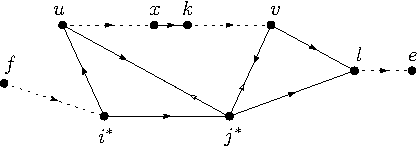
\includegraphics[width=0.8\textwidth]{figures/single/platoon-preservation-proof-diagram.pdf}
  \caption{Sketch of the nodes and most important arcs used in the proof of
    Proposition~\ref{prop:exhaustive}. Dashed arcs represent chains of
    unspecified length. The two open arrows indicate the new direction of their
    arc under ordering $\pi'$.}\label{fig:platoon-preservation-diagram}
\end{figure}


\section{Implementation details}

We have an \texttt{ActionTransform} base class with implementations
\texttt{PaddedEmbeddingModel} and \texttt{RecurrentEmbeddingModel}. The
\texttt{ActionTransform} class takes care of transforming actions in terms of
staying on the same lane or moving to the next lane to actions in terms of
absolute lane identifiers. Specifically, \texttt{action\_transform()} takes a
logit of the binary choice model and outputs a lane identifier and
\texttt{inverse\_action\_transform()} takes a lane identifier and outputs either
zero or one.
%
Both embedding models have a \texttt{state\_transform()} method that constructs
a numerical observation tensor based on the state encoded in the automaton, as
explained in Section~\ref{sec:neural}.
%
Figure~\ref{fig:state-action-transforms} shows an overview of the state and action transform functions and how
they are related to each other.
%
We explicitly store the length of the
horizon as the first entry of the tensor. Maybe we should use the
\texttt{torch.nn.utils.rnn.pack\_sequence()} function that is available in
\texttt{torch}.

\begin{figure}[h]
  \centering
  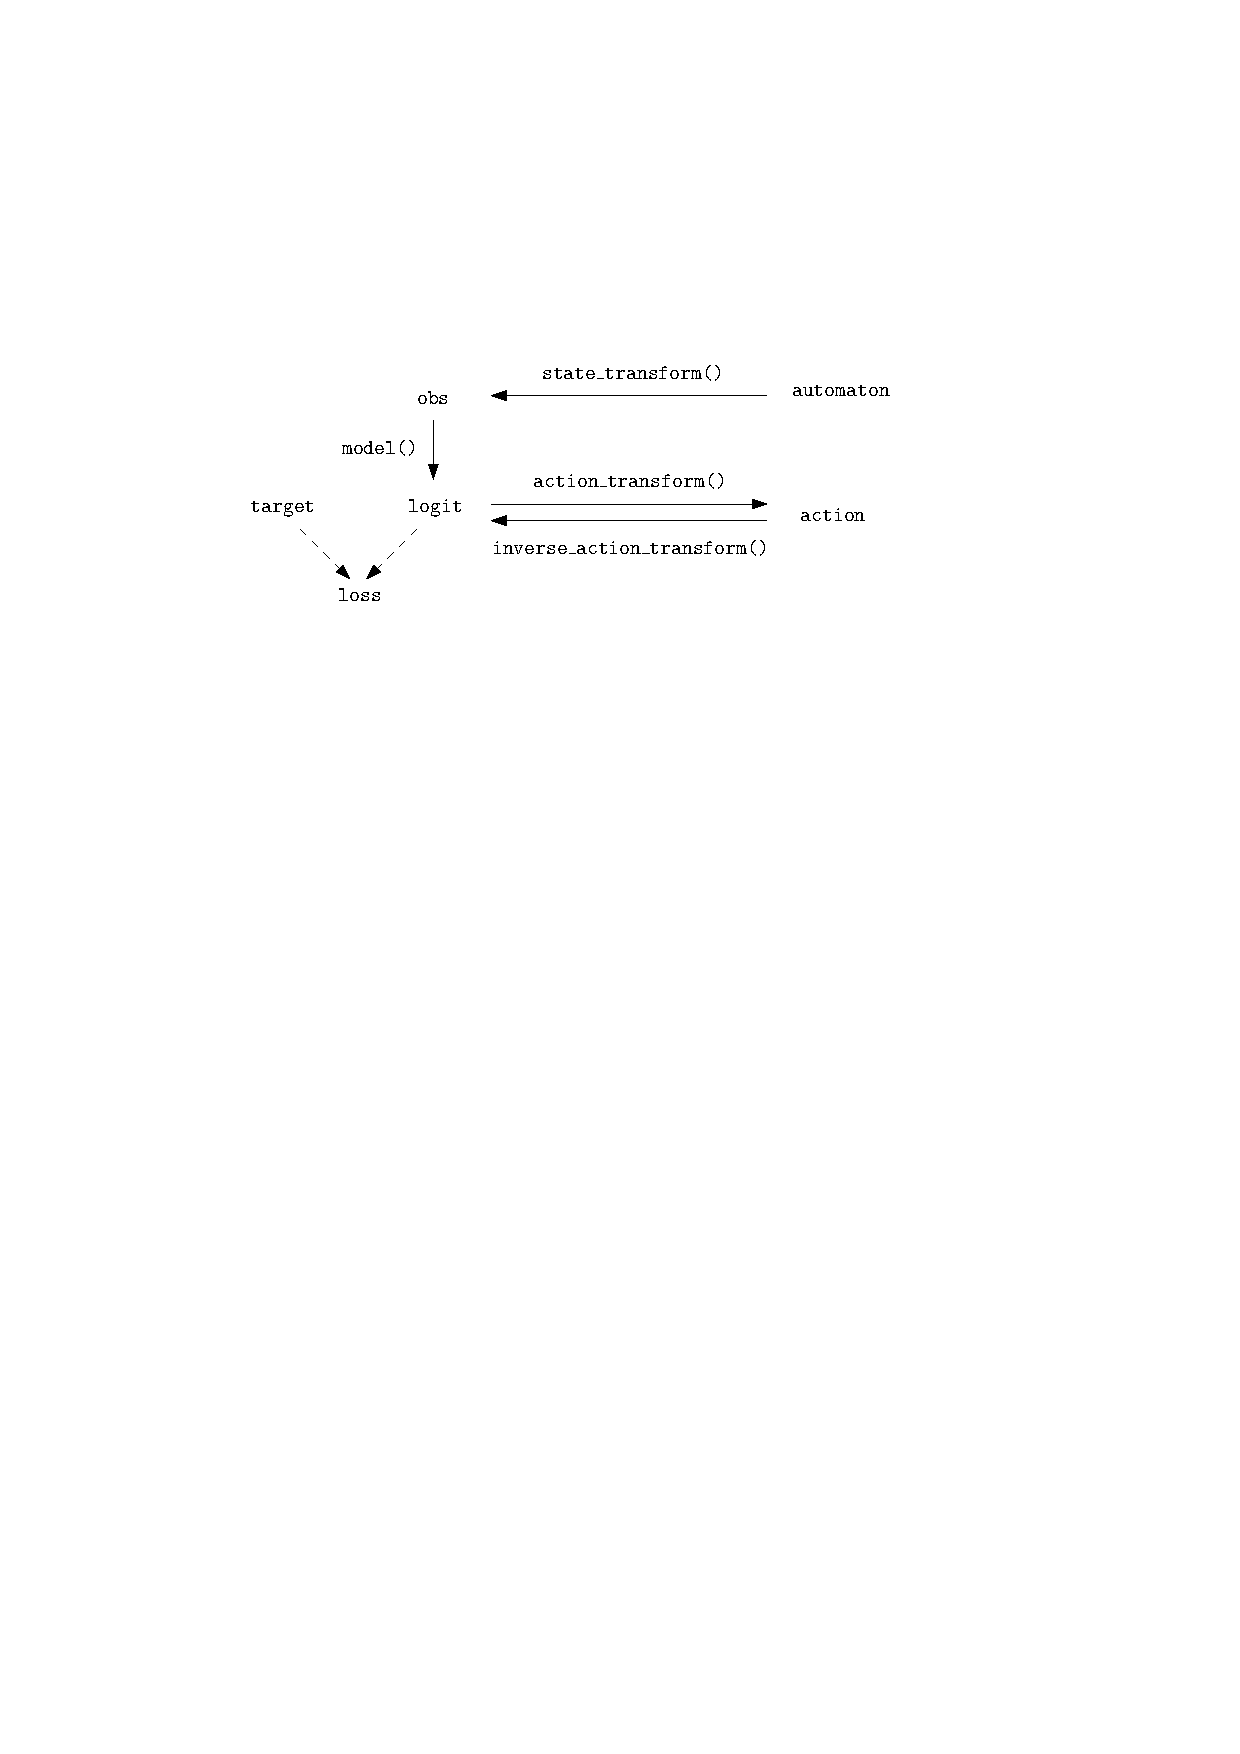
\includegraphics[scale=1]{figures/state_action_transforms}
  \caption{Schematic of the state and action transform functions used for
    imitation learning. Given some optimal state-action training pair, the
    \texttt{target} logit is computed from the optimal action using the inverse
    action transform.}
  \label{fig:state-action-transforms}
\end{figure}


\newpage


\begin{figure}
  \centering
  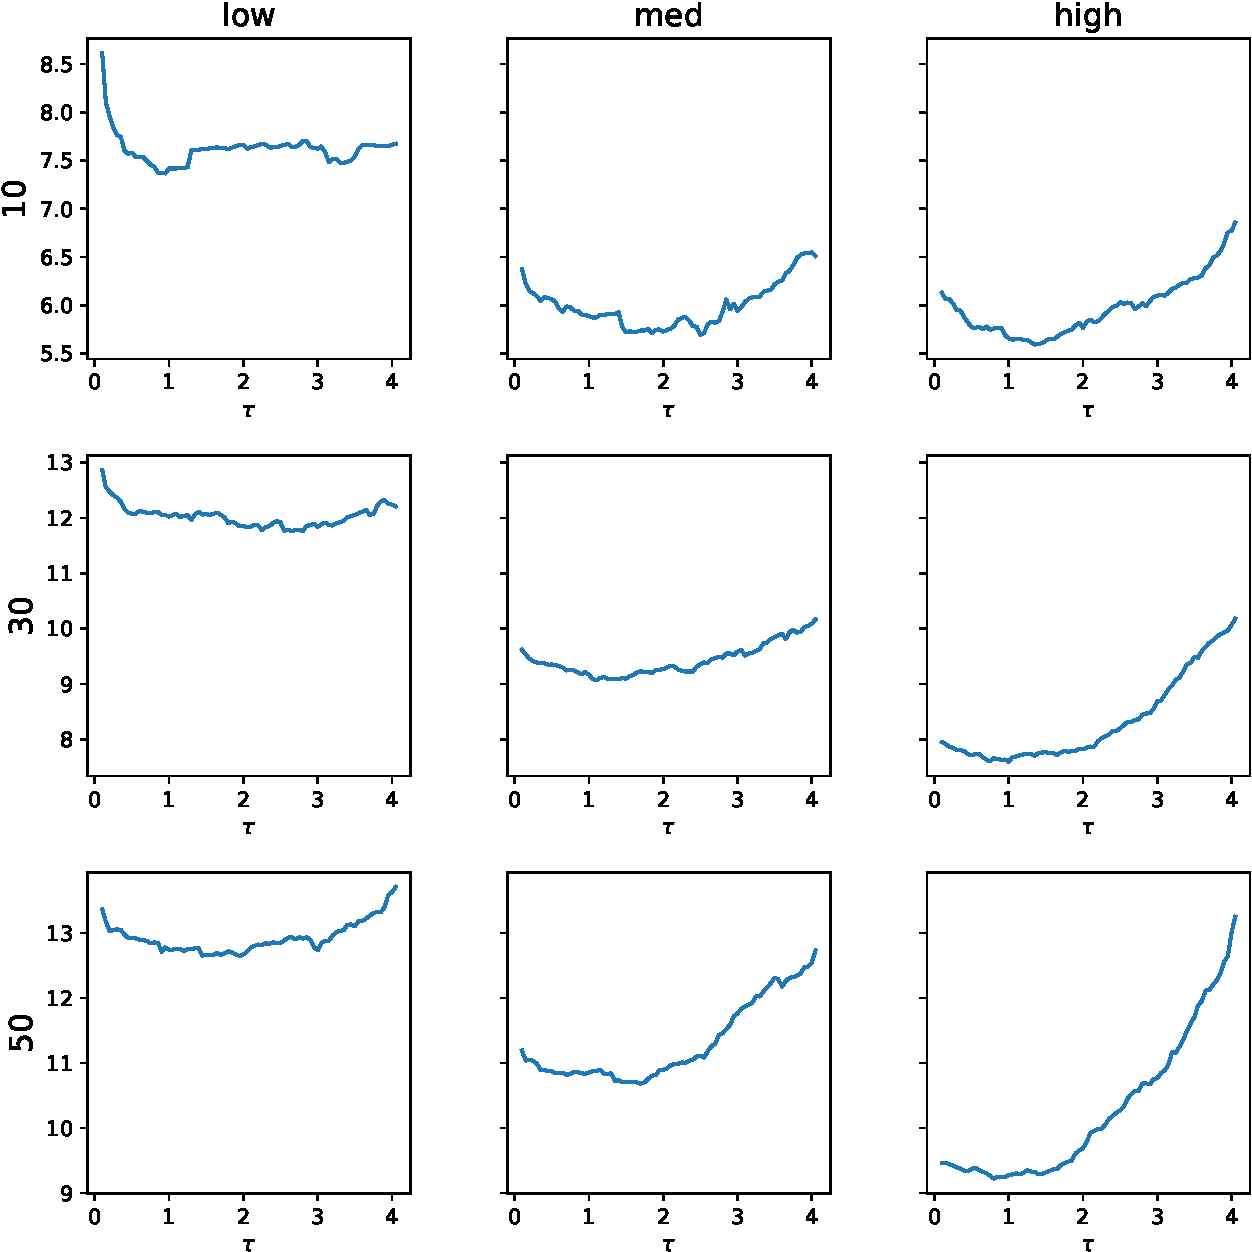
\includegraphics[width=0.9\textwidth]{figures/single/tau_fit.pdf}
  \caption{Charts to verify threshold heuristic model fit. For each indicated
    instance training set, the average delay
    $\sum_{s \in \mathcal{X}} \textrm{obj}(y_{\tau}(s)) \, / \, {|\mathcal{X}|}$
    is plotted as a function of the threshold $\tau$. We use these plots to
    verify that the range of possible candidates for $\tau$ has been chosen wide
    enough, which is probably the case when the graphs are somewhat smooth and
    convex. Observe that larger instances show smoother curves. Furthermore,
    observe that the class of instances with high arrival intensity shows an
    apparent optimal value of $\tau$ around $1$, which might be related somehow
    to our choice of $\sigma = 1$.}
  \label{fig:tau_fit}
\end{figure}

\begin{figure}
  \centering
  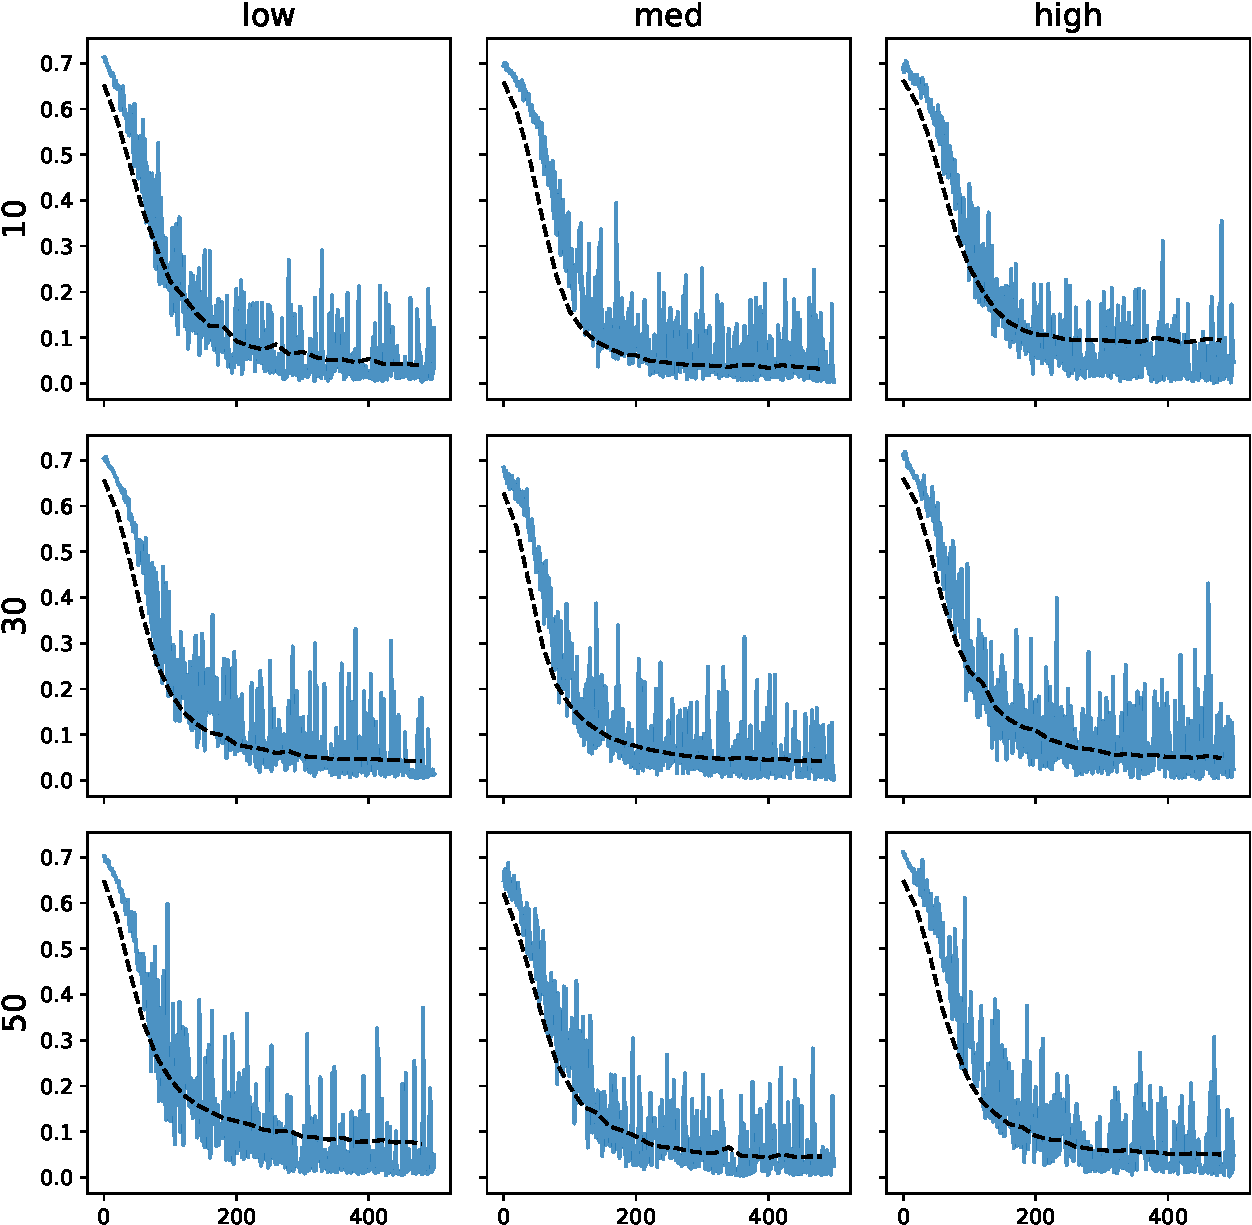
\includegraphics[width=0.9\textwidth]{figures/single/neural_fit.pdf}
  \caption{Loss plots to verify neural heuristic model fit. For each indicated
    instance training set, the training loss is plotted for each training step
    in blue and the validation loss is plotted as the dashed line. Recall that
    the validation loss is the average binary cross entropy loss after a given
    number of training steps. The training loss is plotted for each individual
    step without smooting.}
  \label{fig:neural_fit}
\end{figure}

\end{document}

% to enable the minted package
% Local Variables:
% TeX-command-extra-options: "-shell-escape"
% End:
